\newpage
\subsection{Kommunikation}\label{subsec: Kommunikation} 
\subsubsection{WLAN Konfiguration}\label{subsub: Wlan Konfiguration}
Die Funkkommunikation zwischen Sensor, Aktor und MQTT-Brocker wird mittels Wireless Local Area Network (WLAN) auf dem OSI layer 1 statt finden. Um die einzelnen Target also Sensoren und Aktoren in das Lokale Netzwerk zu verbinden, wird beim Starten des Mikrocontrollers ein Accespoint eröffnet. Für den Wifi-Configurations Prozess wird die entsprechende Bibliothek eingebunden. Diese steht auf Github zur Verfügung \cite{zhouhan0126_zhouhan0126/wifimanager-esp32_2019}. 

\begin{figure}[H]
	\centering
	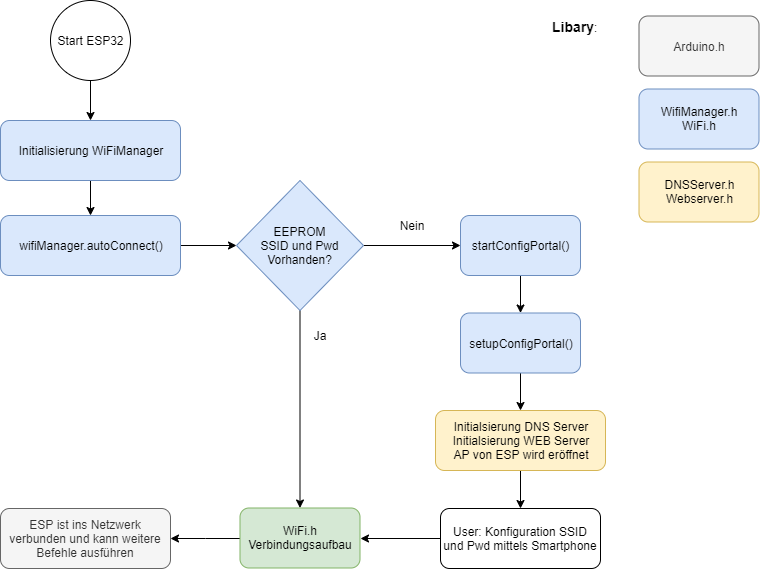
\includegraphics[width=\textwidth]{graphics/statediagramWiFi.png}
	\caption{Statediagram Verbindungsaufbau ESP ins Netzwerk mit einem AP}
	\label{pic: statediagramWiFi}
\end{figure}   

Wird die Bibliothek WiFiManager.h eingebunden und initialisiert stehen verschiedene Funktionen zur Verfügung. Die Funktion autoConnect() eröffnet nach dem Start des Mikrocontrollers einen Access-Point, wenn keine Konfigurationsdaten im nichtflüchtigen Speicher sind. Falls Konfigurationsdaten vorhanden sind, werden sie aus dem EEPROM gelesen und es wird kein Access-Point eröffnet.   

Mit einem Gerät beispielsweise Notebook oder Smartphone kann in den Netzwerk Einstellungen der Mikrocontroller mit dem Name 'Aktor' oder 'Sensor' mit anschliessender Chip-ID gefunden werden. 
Sobald "verbinden" mit diesem Netzwerk gewählt wird, startet der Webbrowser eine Konfigurationsseite. 

\begin{figure}[H]
	\centering
	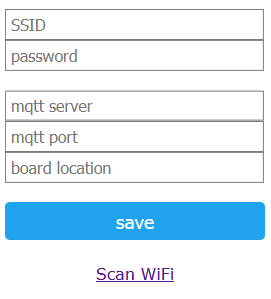
\includegraphics[width=0.3\textwidth]{graphics/Configportal2.PNG}
	\caption{Wifi Konfiguration Portal}
	\label{pic: Configportal}
\end{figure}   

Wird 'Scan Wifi' betätigt werden Netzwerke, welche in der Umgebung gefunden wurden, angezeigt, die Parameter die zur WiFi Verbindung notwendig sind, können nun eingegeben werden. Im unteren Teil wird die MQTT-Brocker-Adresse und der Port eingegeben. Als `board-location' soll der Standort des Gerätes eingegeben werden, aus dieser Eingabe werden MQTT-topics generiert. 

\begin{figure}[H]
	\centering
	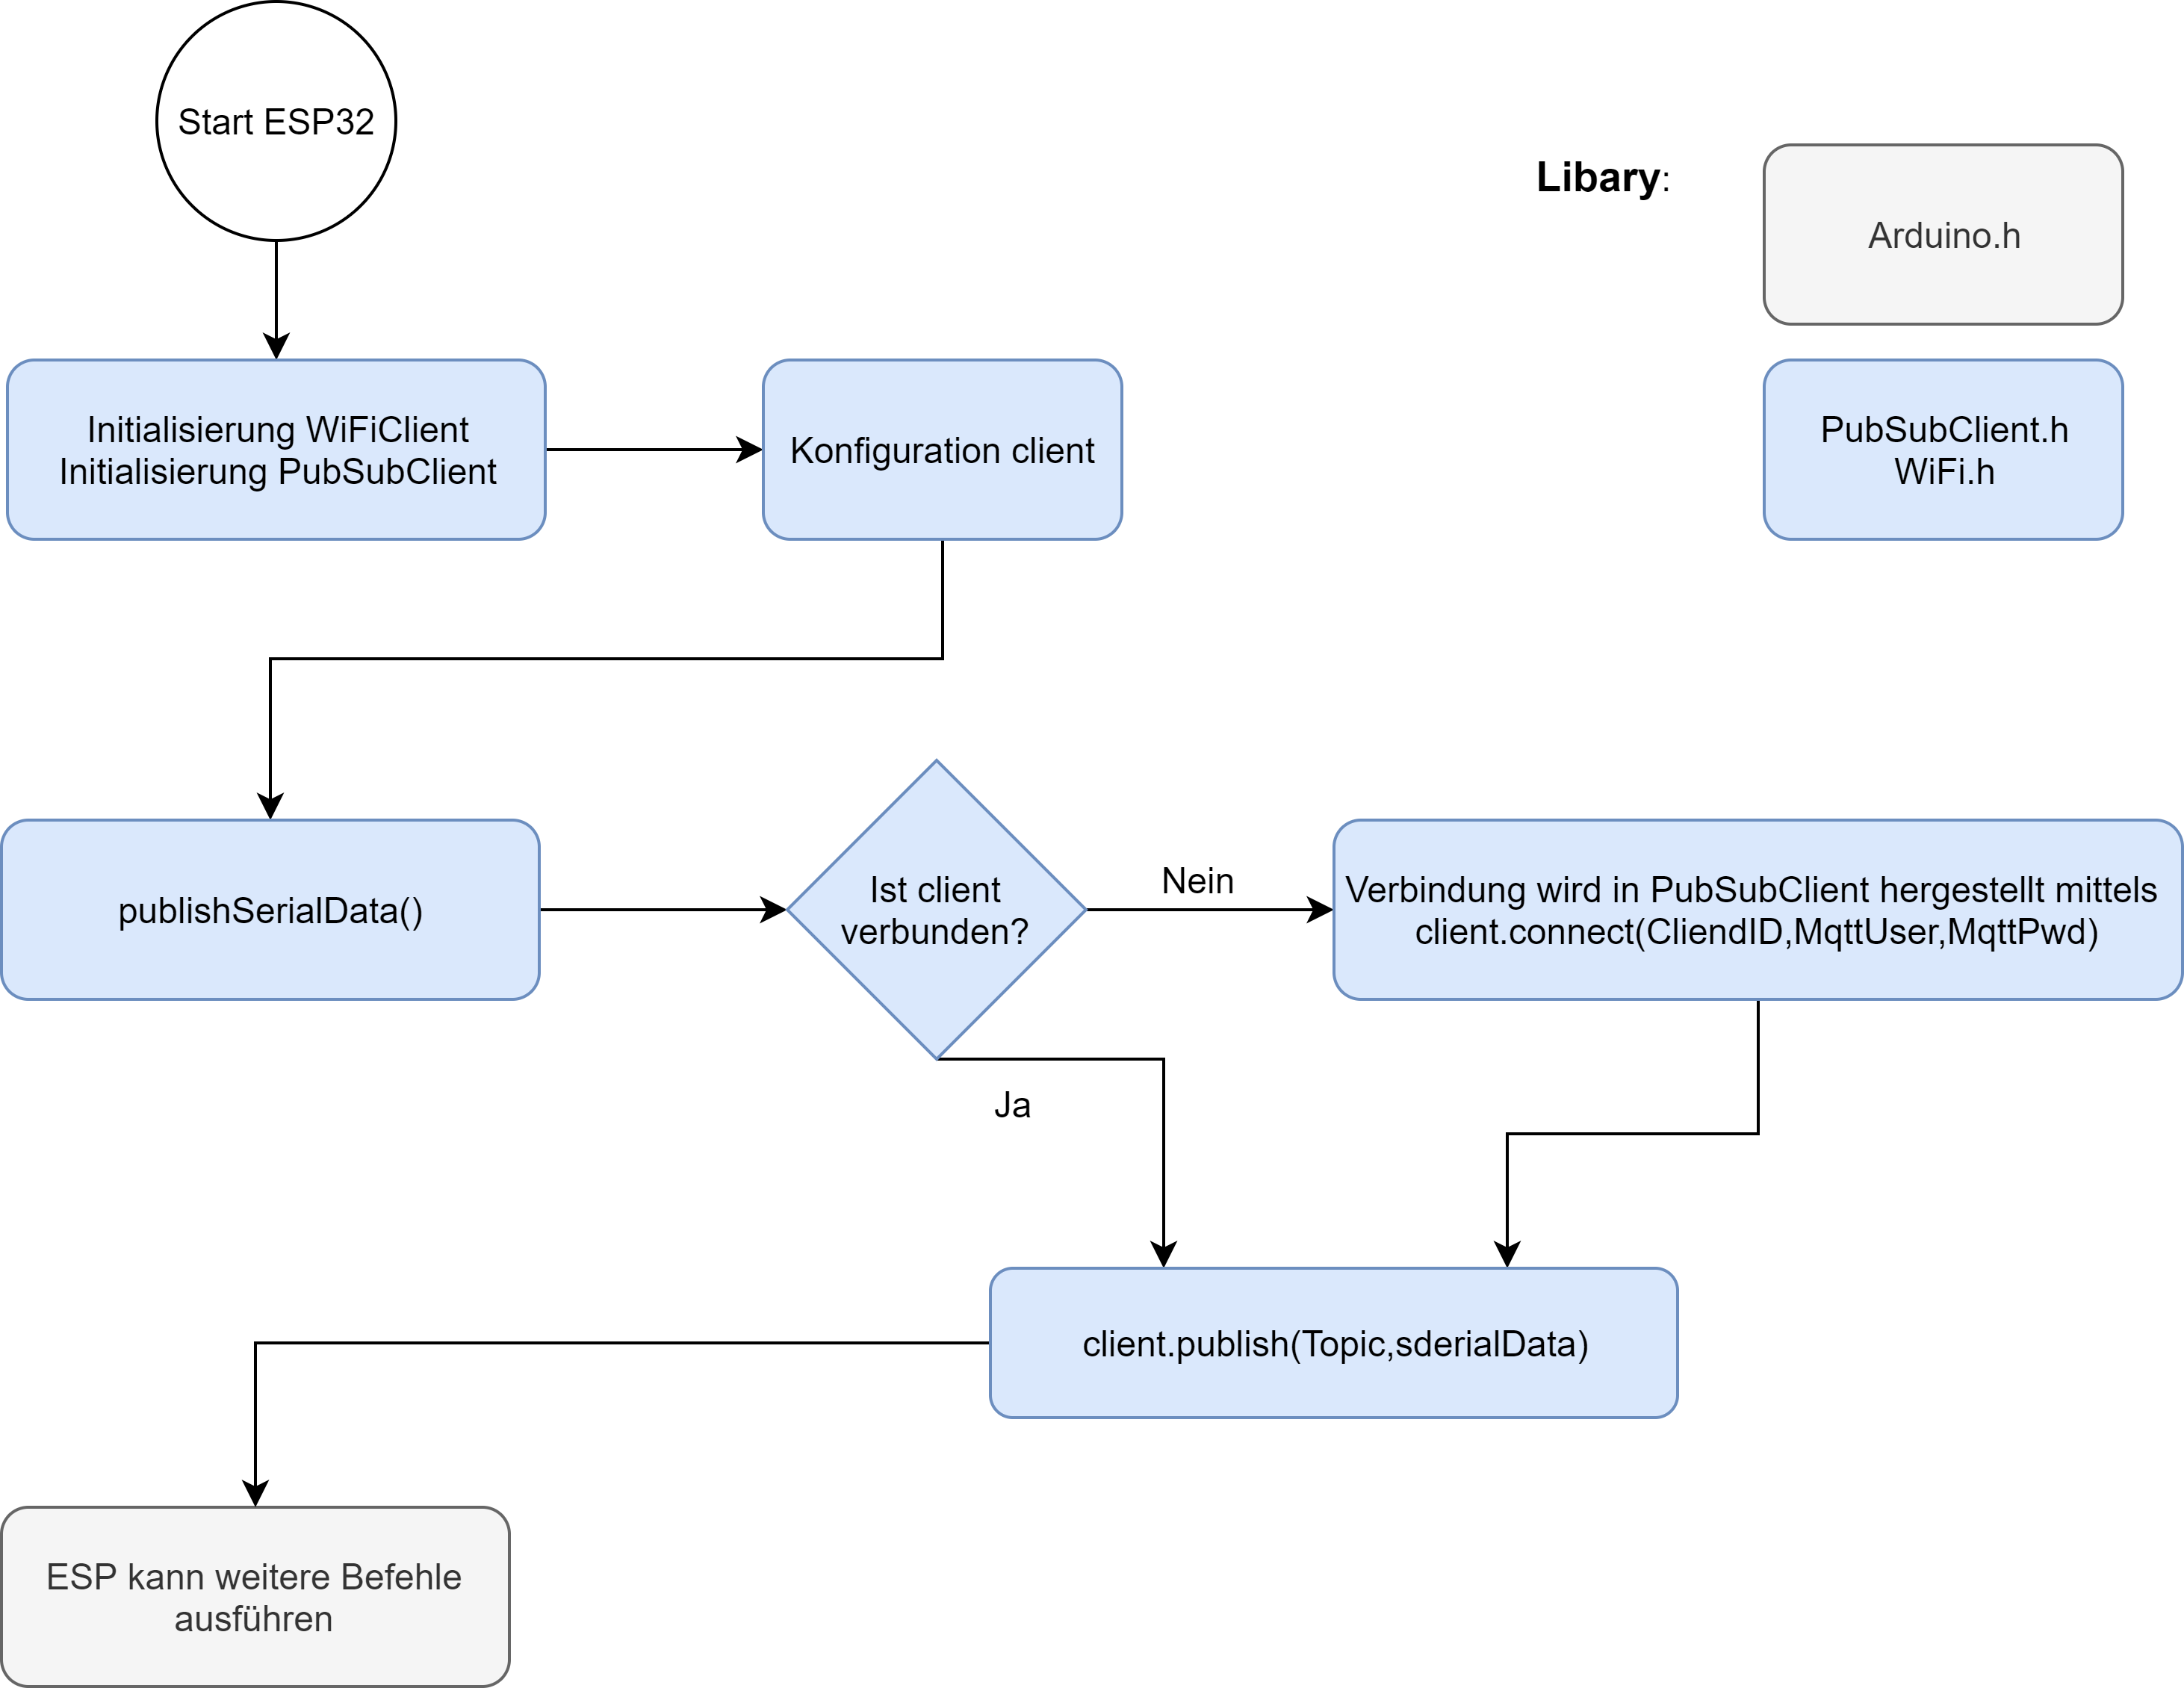
\includegraphics[width=\textwidth]{graphics/MQTTSubPubClient.png}
	\caption{Esp Info}
	\label{pic: SubPubClient}
\end{figure}   

Die für die MQTT-Kommunikation wird die Libary PubSubClient.h eingebunden. Als erstes wird der WiFiClient initialisiert. 

Danach wird der PubSubClinet als Client instanziiert, für diesen Vorgang werden folgende Parameter benötigt:\\
\begin{itemize}
\item 	server: Adresse von MQTT-Server\\
\item 	port: der Port von dem MQTT-Server\\
\item 	client: eine Instanz vom Ethernet-Client.\\
\end{itemize}
Die Funktion publishSerialData() ermöglicht, eine Nachricht zu veröffentlichen, bei diesem Vorgang wird den Topic und die Payload veröffentlicht. Beim Aufruf dieser Funktion, wird jedes mal überprüft ob die Verbindung zum MQTT-Broker in Ordnung ist. 

Ist die Verbindung nicht in Ordnung, wird sie mit der Funktion reconnect() hergestellt.

Ist die Verbindung in Ordnung werden die Daten mit dem Befehl publish() veröffentlicht \cite{noauthor_arduino_nodate-1}.

\subsection{Programmcode Sensorbord}
Die Aufgabe welcher der Mikrocontroller vom Sensorboard  übernehmen besteht darin, dass er Betätigungen der Touchtasten auf dem Frontprint erkennt. Jeder Touchtaster besitzt ein LED mit dem das Betätigen bestätigt wird. Diese Funktion wurde so initialisiert, damit der User eine sofortige Kenntnis über die ausgelöste Aktion bekommt. Mit dem Sensorboard wird auf dem Frontprint die Umgebungstemperatur gemessen.



\subsubsection{	Übersicht} 
\begin{figure}[H]
	\centering
	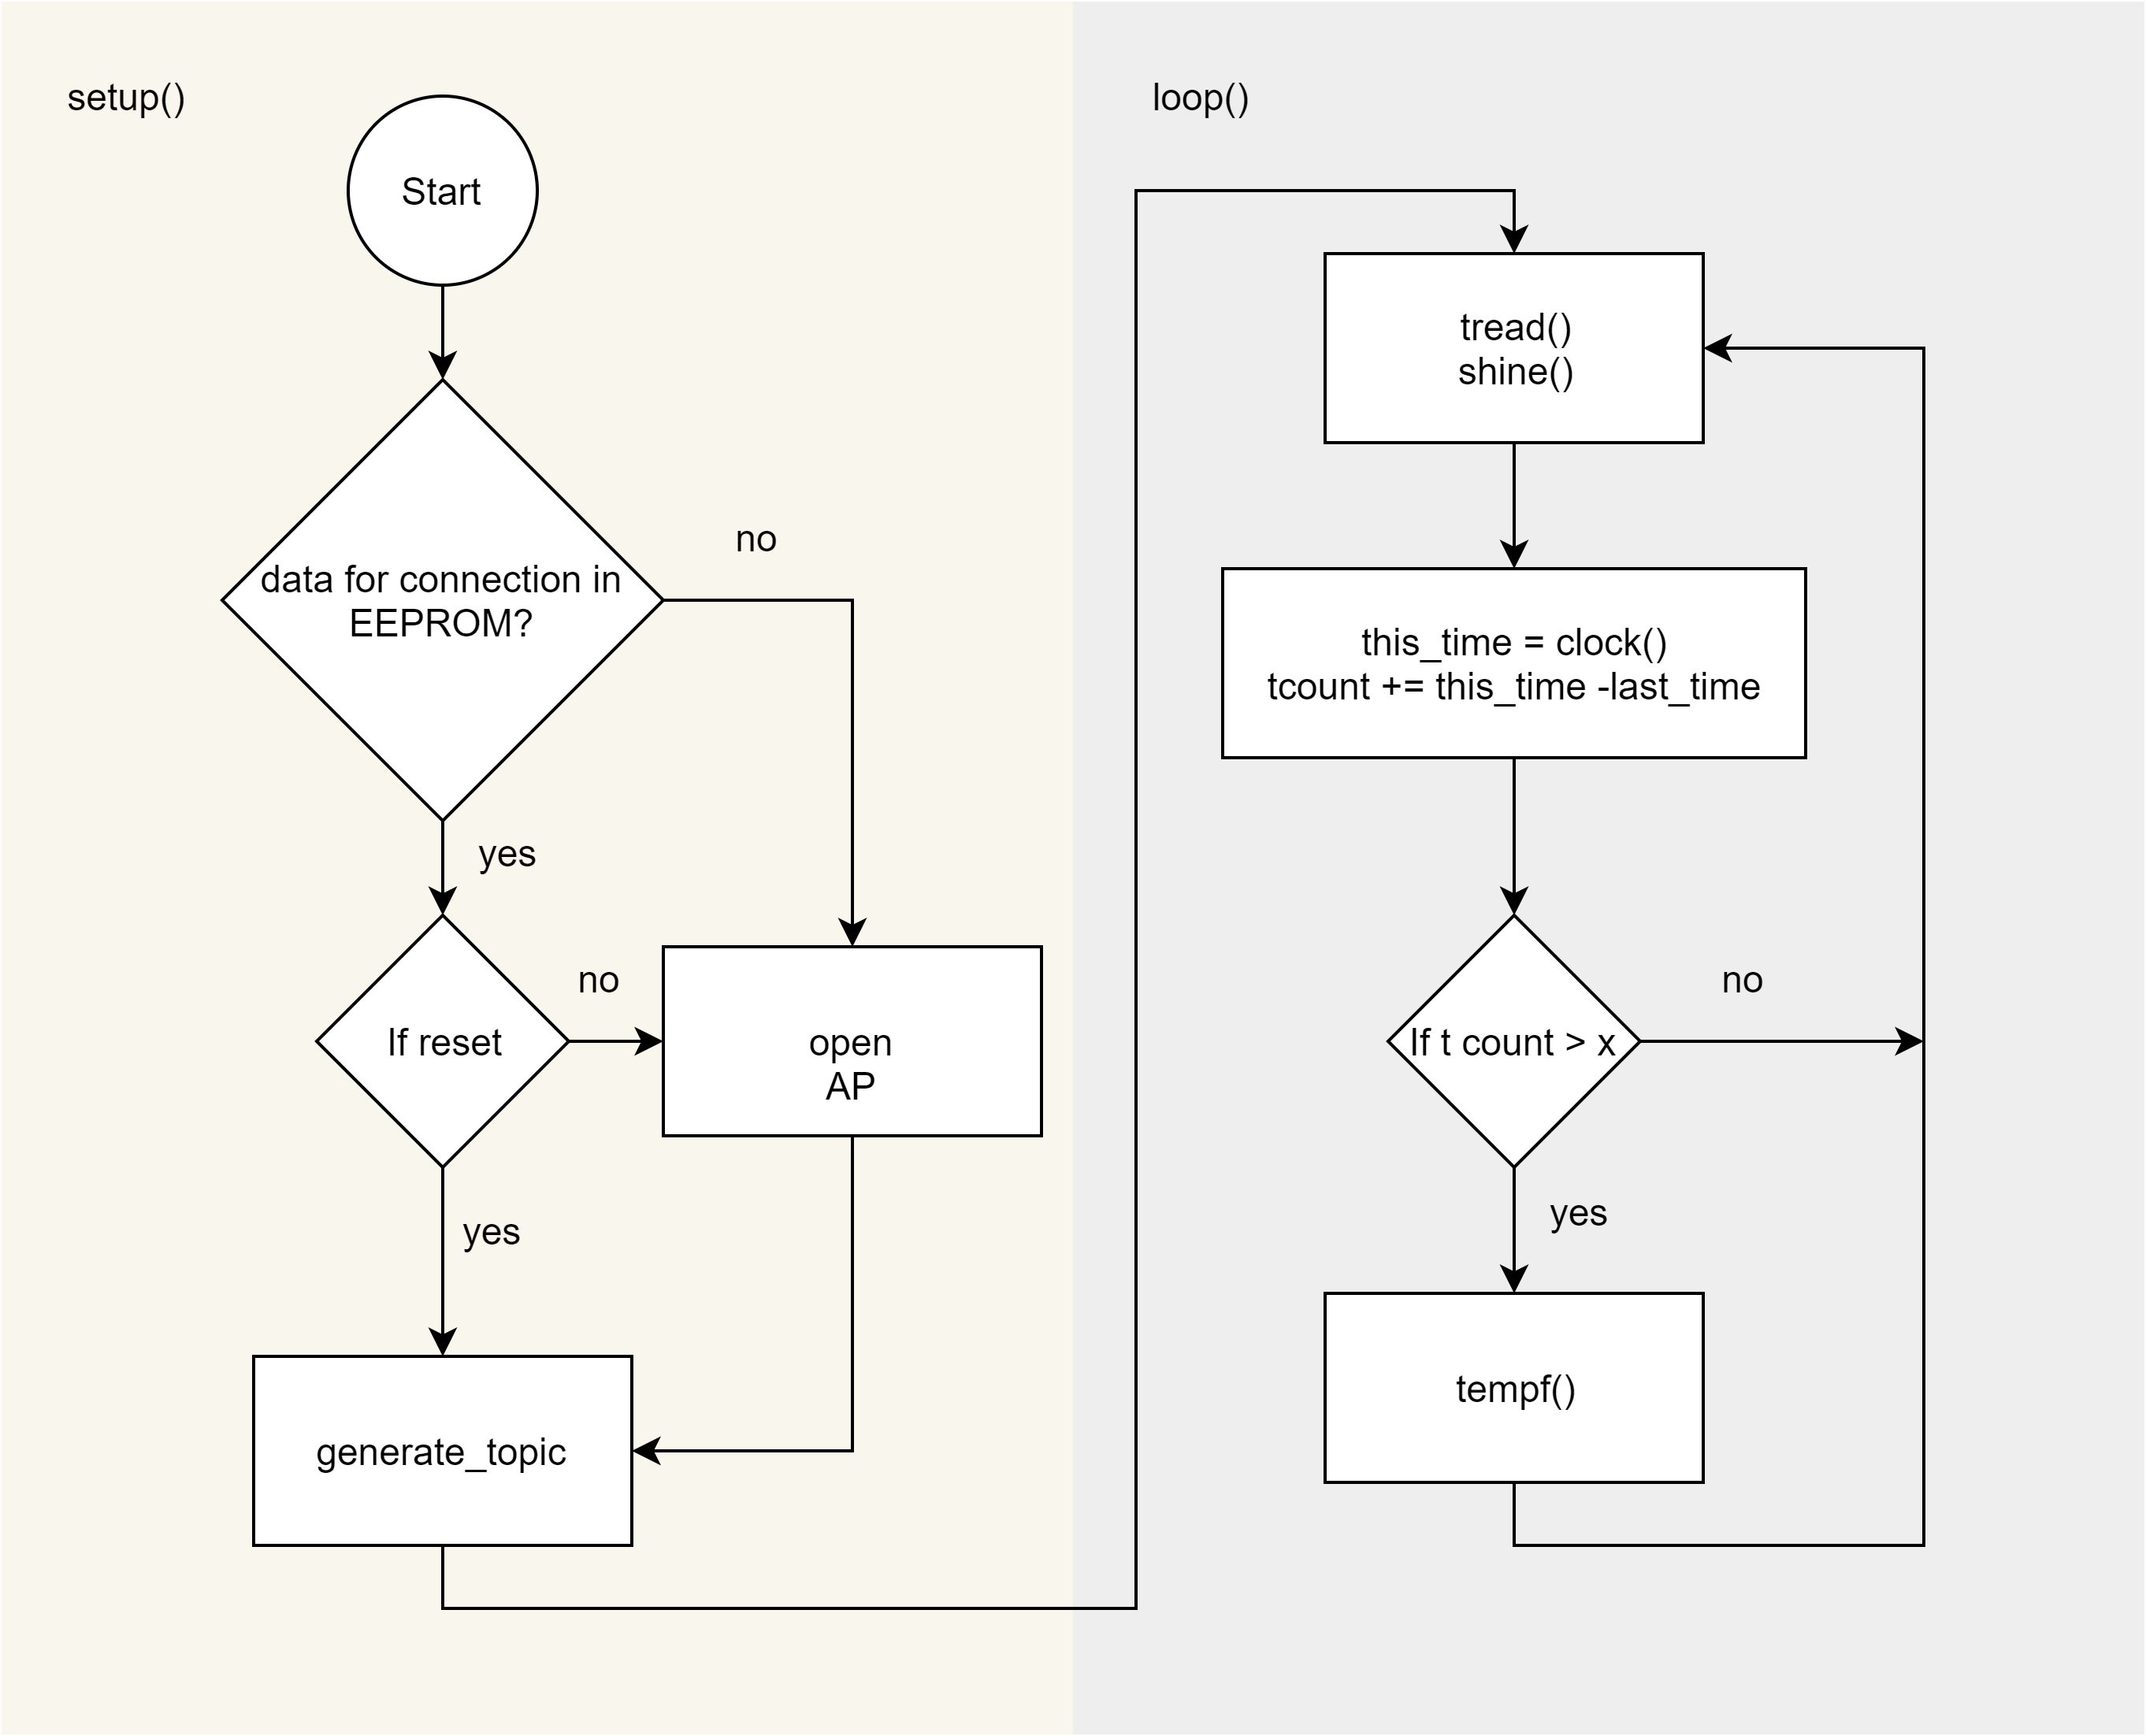
\includegraphics[width=\textwidth]{graphics/StatemaschineSensor.png}
	\caption{In dieser Abbildung ist das Statediagram vom Sensorboard abgebildet}
	\label{pic: statemaschine sensor}
\end{figure} 

\newpage

\subsubsection{setup()}\label{subsubsec: sensor setup}
Wird der Mikrocontroller gestartet so werden als erstes Configurations-Daten im EEPROM gesucht. Werden keine Daten gefunden oder wird die Reset-taste betätigt wird ein Accespoint eröffnet und Confugurations Parameter können mittels Browser eingegeben werden. Dieser Vorgang wird im Kapitel Kommunikation genauer beschrieben. Als nächster Schritt werden für die MQTT-Messages die Topics anhand der Bordbezeichnung und der Anwendung generiert. Die Bordbezeichnung wird im Configportal eingegeben und im EEPROM abgespeichert, sie dient dazu, wenn mehrere Boards installiert werden um die empfangenen Nachrichten zu unterscheiden. Eine mögliche Topic für eine MQTT Nachricht wenn beispielsweise der erste Taster betätigt wird kann folgendermassen aussehen: "data/sesnorboard/wohnzimmer/S1" in diesem Fall wurde die Bordbezeichnung Wohnzimmer gewählt. 

\subsubsection{loop()} \label{subsubsec: sensorloop}
Im loop() wird als erstes die Funktion tread(), dann shine() aufgerufen, danach wird die Momentane Zeit mit der Funktion clock() geholt. In der Variabel count wird die Zeitdifferenz zwischen den wiederholenden Durchgängen von touch() addiert. Dies passiert solange bis der Wert x erreicht ist, in diesem Fall alle 10 Sekunden. Wenn der Wert x erreicht ist wird die Funktion tempf() aufgerufen, mit dieser wird mittels NTC die Temperatur gemessen. Im gleichen Zyklus wie die Temperaturmessungen Durchgeführt werden, wird die Staus LED geschaltet, so kann überprüft werden, ob sich das Bord im normalen Betrieb befindet, sprich der loop() wird gewiss komplett Durchlaufen. Die Funktionen sind in der nachfolgenden Abbildung abgebildet und werden anschliessend erläutert.

\begin{figure}[H]
	\centering
	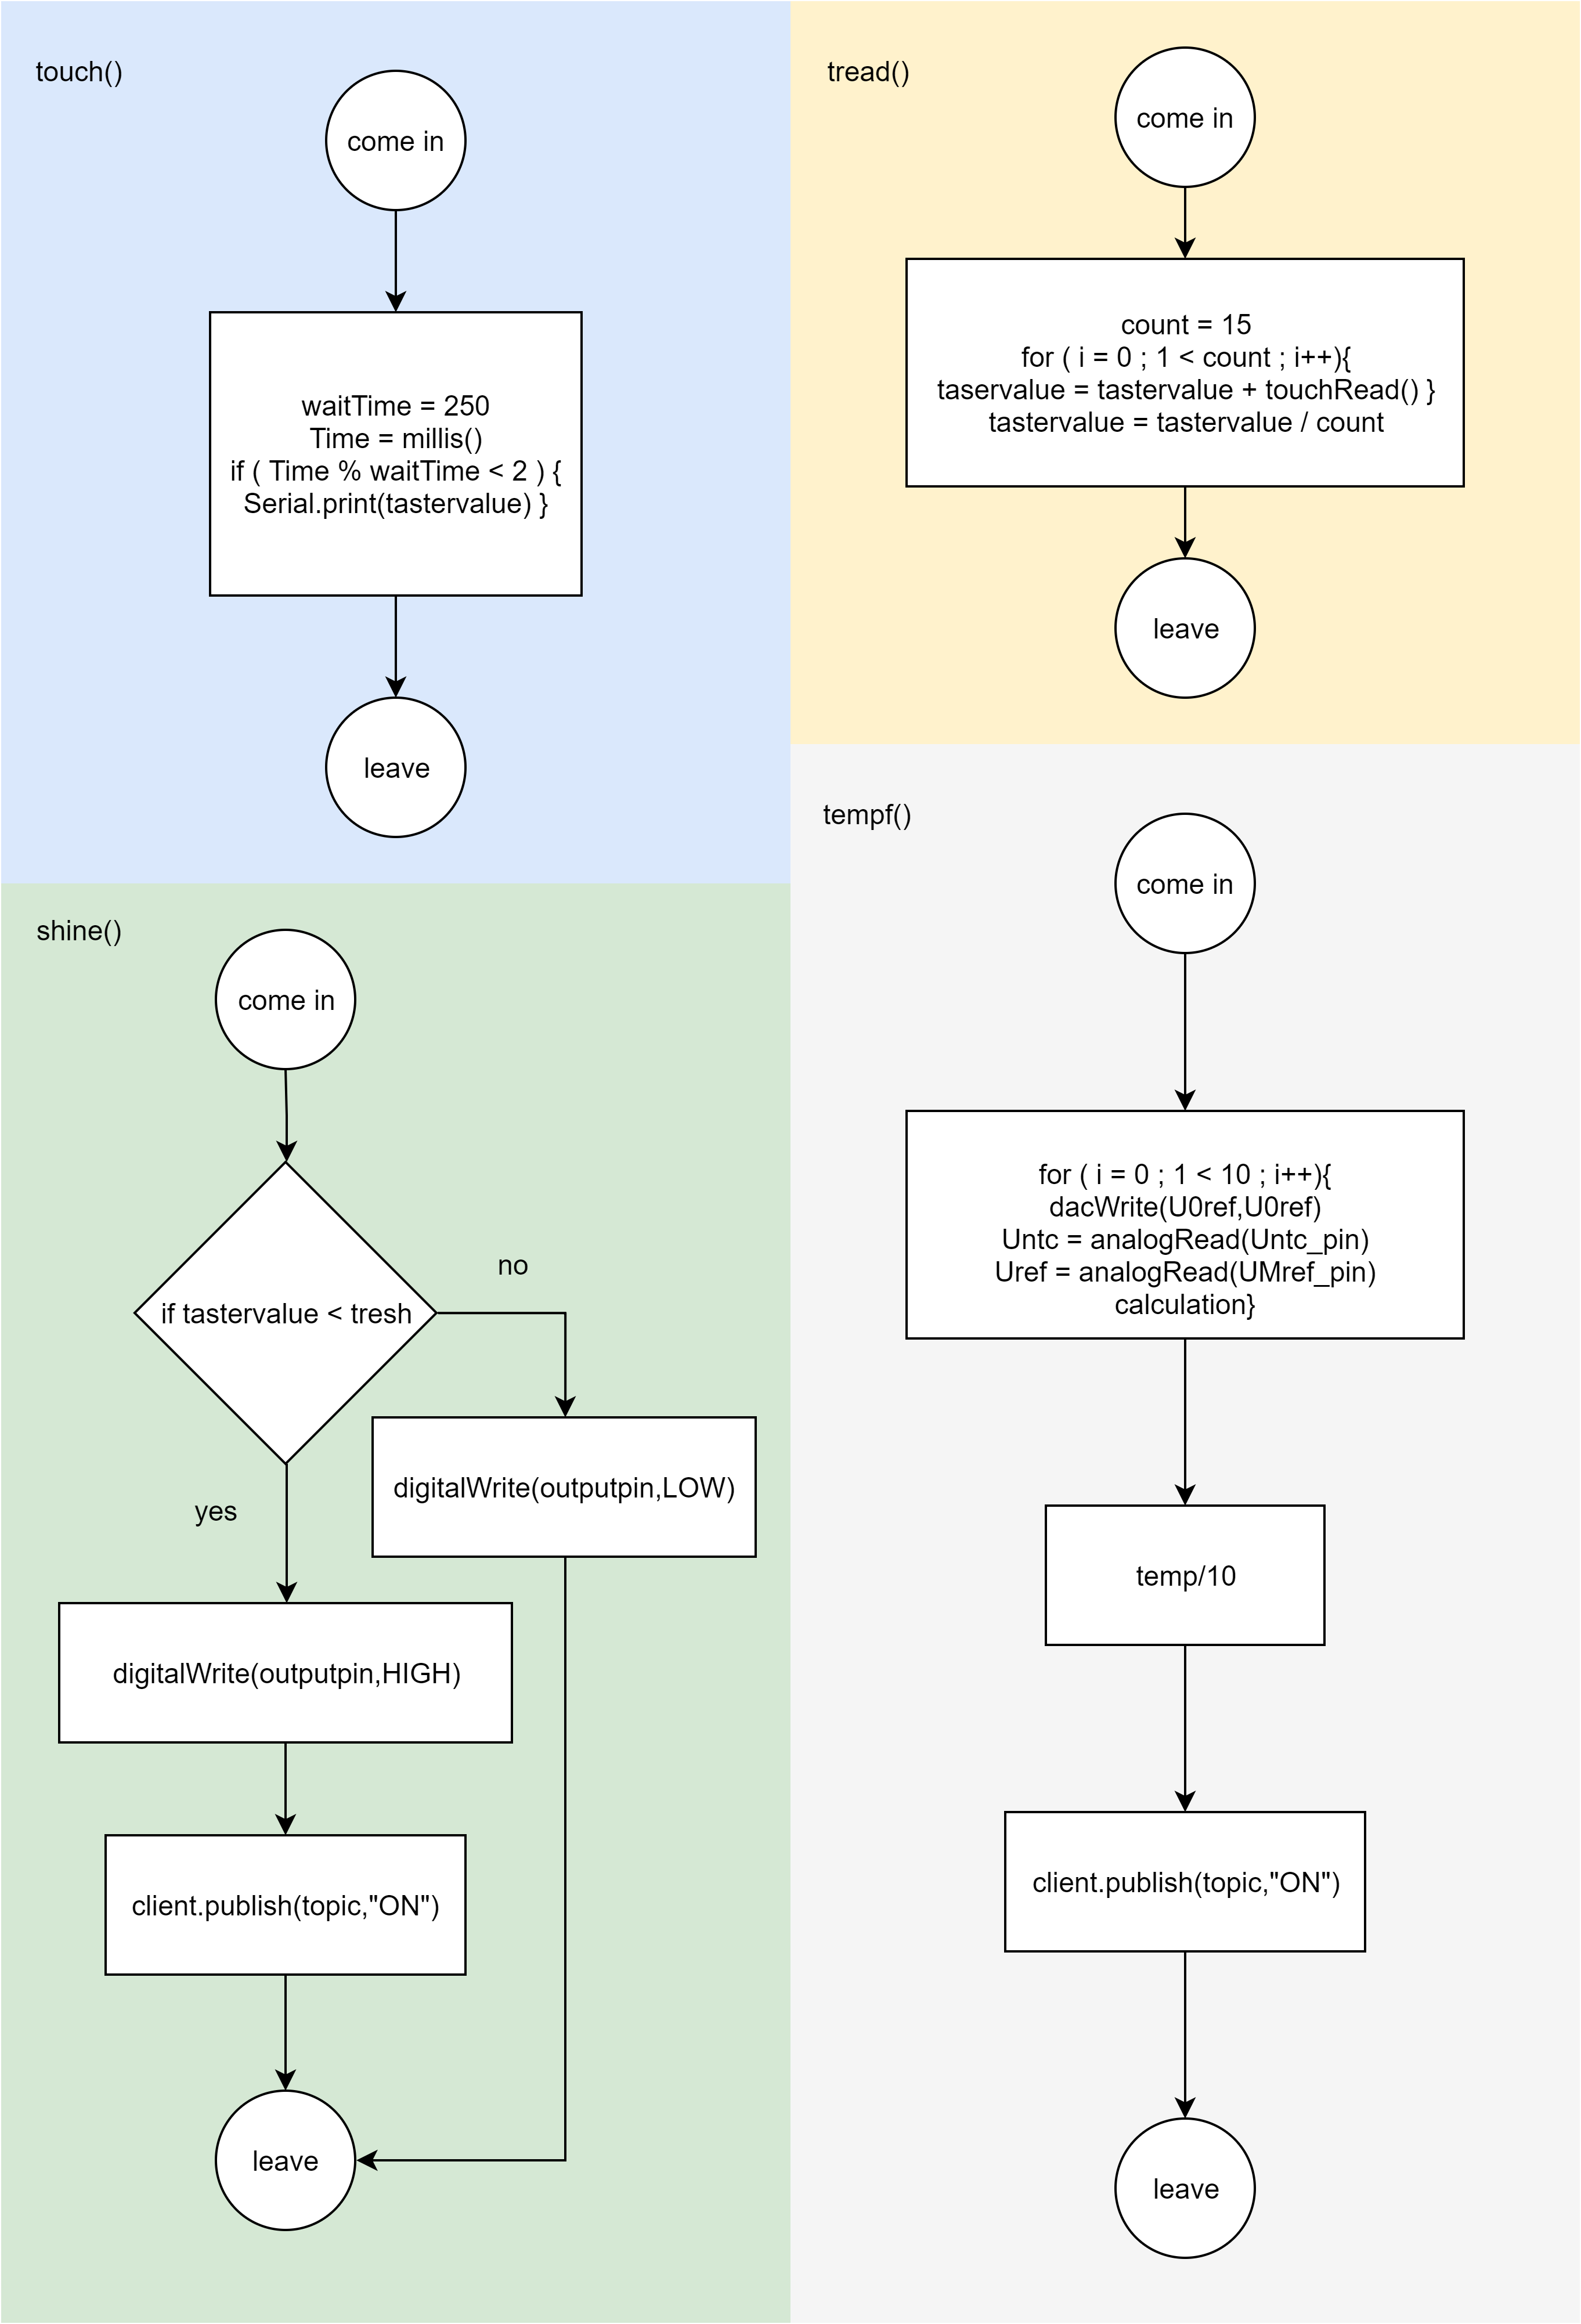
\includegraphics[width=\textwidth]{graphics/FunktionenSensor.png}
	\caption{In dieser Abbildung sind die Funktionen vom Sensorboard abgebildet}
	\label{pic: funktionen sensor}
\end{figure}   
\subsubsection{touch()} 
Wie in der Abbildung \ref{pic: statemaschine sensor} zu erkennen ist, wird die Funktion touch() nicht aufgerufen. Sie dient alleine zum debuggen also um den optimalen tresh Wert zu finden. Dieser Wert definiert ab wann die Touchsensoren als gedrückt erkannt werden. In der Funktion wird die Variabel waitTime initialisiert mit dem wert 250 weiter wird der Wert millis() in die Variable Time gesetzt. In einer for-wihle werden so lange Time modulo waitTime kleiner als 2 sind, sprich die ersten 2 Millisekunden von 250 Millisekunden, mit Serial.println() der aktuell eingelesene Touchwert ausgegeben. Dieser Wert befindet sich im Ruhezustand um 50-80, wenn eine entsprechende Touch-Taste betätigt wird sinkt dieser Wert auf 10-30.  
\subsubsection{shine()}
In der Funktion shine() wird in einer for-while der Eingelesene Wert das sogenannte taservalue der jeweiligen Touchtasten mit dem Tresholdwert, tresh verglichen. Ist das tastervalue kleiner als tresh, wird eine MQTT-Message mit der entsprechenden Topic und der Payloud "ON" published. Ebenso wird die Led der entsprechenden Taste HIGH gesetzt. Trifft der andere Fall zu, wenn das tastervalue grösser als tresh ist wird die entsprechende Led LOW gesetzt.
\subsubsection{tread()}
In der Funktion tread() werden in einer for-while die aktuellen Werte der vier Touch-Tasten eingelesen und in den int-array tastervalue gesetzt, um Ausreisser zu eliminieren, wird ein Mittelwert erstellt. Es werden jeweils 15 Messungen addiert und aschliessend durch die Anzahl Messungen dividiert.  
\subsubsection{tempf()} \label{tempf}
In dieser Funktion wird die Temperatur mit dem NTC ermittelt. So wird als erstes $U_{ref}$ und $U_{ntc}$ als ADC-Wert eingelesen und über 10 Werte gemittelt. Danach wird eine Geradengleichung (Gl.: \ref{eq: U_ADC_sensor}) verwendet, um die ADC-Werte in eine Spannung zu konvertieren. Wie im Kapitel \ref{Temperatursensor} beschrieben und in der Abbildung \ref{pic: Temperatursensor} ersichtlich, bildet ein Vorwiderstand von 100\,K$\Omega$ und der NTC einen Spannungsteiler an dem $U_{ref}$ angelegt wird und am NTC die Spannung $U_{ntc}$ gemessen wird. Aufgrund dessen wird der Widerstand des NTCs $R_T$ mit \ref{eq: R_T} berechnet. Für $U_{ref}$ wird maximal eine Spannung von 2.5\,V verwendet, da der ADC danach nicht mehr linear ansteigt, diese Spannung wird mithilfe eines DACs im Setup() ausgegeben. Die Temperatur in Kelvin ergibt sich dann aus der Gleichung \ref{eq: T}, von dieser Zahl wird danach 273.15 abgezogen, um den Wert in °C zu kriegen. Die angesprochene Gerade (Gl.: \ref{eq: U_ADC_sensor}) ist so ausgelegt, dass sie in dem Spannungsbereich der Temperaturmessung funktioniert. Um sie auszulegen und gleichzeitig die Temperatur zu verifizieren wurde folgendes Verfahren angewendet. Als erstes wurde der Temperaturbereich festgelegt, welcher von -5\,°C bis +45\,°C reicht. Dann wurde mittels eines Klimaschrankes \ref{pic: Klimaschrank} die Temperaturen in 5\,°C $\pm$1°C Schritten festgelegt. Um die Temperatur genauer zu messen wurde ein NiCr-Ni Temperaturfühlers (Messgerät Therm 2250-1) verwendet. Der Sensorbaustein und der Temperaturfühler werden nun verschiedenen Temperaturen ausgesetzt und der Sensorbaustein gibt seine ADC-Werte weiter (Tabelle: \ref{tab: Temp_ADC}). Es wurde festgestellt, dass $U_{ref}$ annäherungsweise über die Temperatur konstant bleibt, hier war der ADC Wert 2768\,$\pm$1. $U_{ref}$ wurde ebenso mittels eines Multimeters gemessen und es ergab sich eine Spannung von U$_{ref}$ = 2.39\,V. Die mit dem NiCr-Ni Temperaturfühler gemessenen Temperaturen wurden mithilfe von Gleichung \ref{eq: R_T,2} und \ref{eq: U_ntc} in Spannungen verrechnet, welche an dem NTC anliegen, falls die Toleranz klein genug sind. Diese theoretischen Spannungen wurden genommen, entgegnen den ADC-Werten gesetzt und einen linearen Fit mit QtiPlot erstellt. Die Gerade (Gl.: \ref{eq: U_ADC_sensor}) kam dabei heraus und sie wurde auf die ADC-Werte der Tabelle \ref{tab: Temp_ADC} angewendet, um dann mithilfe von den Gleichungen \ref{eq: R_T} und \ref{eq: T} die Temperaturen zu berechnen, die der Sensorbaustein schlussendlich anzeigt. Diese berechneten Temperaturen des Sensorbausteins wurden dann den gemessenen Temperaturen des Temperaturfühlers in der Tabelle \ref{tab: Temp_ADC} verglichen, die grösste Abweichung war 0.23\,K bei 39.2\,°C, bei welchen der Sensorbaustein 39.43\,°C anzeigen würde. Der Grund dieses Verfahrens ist, dass $U_{ref}$ leicht unterschiedliche Werte annehmen kann, da der DAC nicht genau ist, vereinfacht gesagt wurde im Bereich von $U_{ref}$ = 2.39\, linearisiert. $U_{ref}$ wird wie $U_{ntc}$ gemessen, was bedeutet dass es keine Rolle spielt ob, $U_{ref}$ = 2.30\,V oder 2.4\,V ist. Im Vergleich zur Kurve in \ref{ADC} berechnet die Kurve für den Sensorbaustein die korrekte Spannung für den ADC-Wert der Referenzspannung, obwohl der Unterschied von 2.38\,V (Gl.: \ref{eq: ref_allgemein}) zu 2.39\,V (Gl.: \ref{eq: ref_sensor}) mit 10\,mV minimal ist. Ein Problem ist, aber dass der Sensorbaustein nun auf die Bedingungen innerhalb eines Klimaschrankes kalibriert wurde, wo die Luft nicht gestanden ist. Wenn die Luft steht wird die Temperatur an der Frontplatte wärmer sein, dies wurde mit einem Korrekturterm gelöst. Vergleichsmessungen mit einem Thermoelement haben ergeben, dass beim NTC die Temperatur um die 2\,°C höher waren, wenn die Luft steht, was auskorrigiert werden muss. In der stehenden Luft wurde 25.6\,°C gemessen und an der Frontplatte 27.6\,°C.
\\
\begin{center}	
Berechnungen zur Temperaturmessung:
\begin{align}
	U &= ADC \cdot m_{sensor} + b_{sensor} \label{eq: U_ADC_sensor}\\
	\frac{R_T}{R_V} &= \frac{U_{ntc}}{U_{ref}\;-\;U_{ntc}} \label{eq: R_T}\\
	T &= \frac{1}{\frac{1}{T_N}+\frac{1}{B} \cdot ln(\frac{R_T}{R_0})}\; 
	\widehat{=}\; \frac{1}{\frac{1}{T_N}+\frac{1}{B} \cdot ln(\frac{R_T}{R_V})}  \label{eq: T}\\
	R_T &= R_0 e^{B\left(\frac{1}{T} - \frac{1}{T_0}\right)} \label{eq: R_T,2}\\
	U_{ntc} &= \frac{R_T}{(R_V + R_T)} \cdot U_{ref} \label{eq: U_ntc}
\end{align}
\\
Konstanten zur Temperaturmessung:
\begin{align*}
	m &= 0.000798\,V \text{(Steigung aus der Geraden von \ref{U_kurve}) als Vergleich}\\
	b &= 0.174\,V \text{(Offset aus der Geraden von \ref{U_kurve}) als Vergleich}\\
	m_{sensor} &= 0.0008155002\,V\\
	b_{sensor} &= 0.1369856\,V\\
	R_V &= 100\,k\Omega\; \text{(Vorwiderstand)}\\
	R_0 &= 100\,k\Omega\; \text{(Widerstand des NTCs bei 25\,°C)}\\
	B &= 4250\,K\; \text{(B-Konstante des NTCs)}
\end{align*}
\\
Variablen zur Temperaturmessung:
\begin{align*}
 U_{ntc}\; &\text{(Spannung über NTC)}\\
 U_{ref}\; &\text{(Spannung über Vorwiderstand und NTC)}\\
 U\; &\text{(Spannung allgemein)}\\
 ADC\; &\text{(ADC-Wert allgemein)}\\
 T\; &\text{(momentante Temperatur in Kelvin)}\\
\end{align*}
\\
Vergleich der Geraden:
\begin{align}
	2.39\,V \widehat{=} 2768;\\
	m_{sensor} \cdot 2768 + b_{sensor} = 2.39 \label{eq: ref_sensor}\\
	m \cdot 2768 + b = 2.3 \label{eq: ref_allgemein}\\
\end{align}
\end{center}

\begin{table}[H]
	\begin{tabular}{|c|c|c|c|}
		\hline
		\textbf{\begin{tabular}[c]{@{}c@{}}Temperatur in °C \\ (Therm 2250-1)\end{tabular}} & \textbf{\begin{tabular}[c]{@{}c@{}}ADC Wert \\ von $U_{ntc}$\end{tabular}} & \textbf{\begin{tabular}[c]{@{}c@{}}Temperatur in °C \\ (Sensorbaustein)\end{tabular}} & \multicolumn{1}{l|}{\textbf{Abweichungen in °C}} \\ \hline
		-4.6 & 2254 & -4.42 & 0.18 \\ \hline
		0.6 & 2119 & 0.65 & 0.05 \\ \hline
		5.6 & 1966 & 5.73 & 0.13 \\ \hline
		10.2 & 1826 & 9.99 & -0.21 \\ \hline
		14 & 1687 & 14.02 & 0.02 \\ \hline
		20.2 & 1474 & 20.02 & -0.18 \\ \hline
		25.1 & 1300 & 24.93 & -0.17 \\ \hline
		29.7 & 1138 & 29.64 & -0.06 \\ \hline
		34.3 & 980 & 34.50 & 0.20 \\ \hline
		39.2 & 832 & 39.43 & 0.23 \\ \hline
		44 & 709 & 43.93 & -0.07 \\ \hline
	\end{tabular}
	\caption{Mit dem Therm 2250-1 aufegenommene Temperaturwerte und die ADC Werte von $U_{ntc}$, welche zu den Temperaturen des Sensorbausteins berechnet wurden, dazu die Abweichungen der Temperaturen voneinander.}
	\label{tab: Temp_ADC}
\end{table}

\begin{figure}[H]
	\centering
	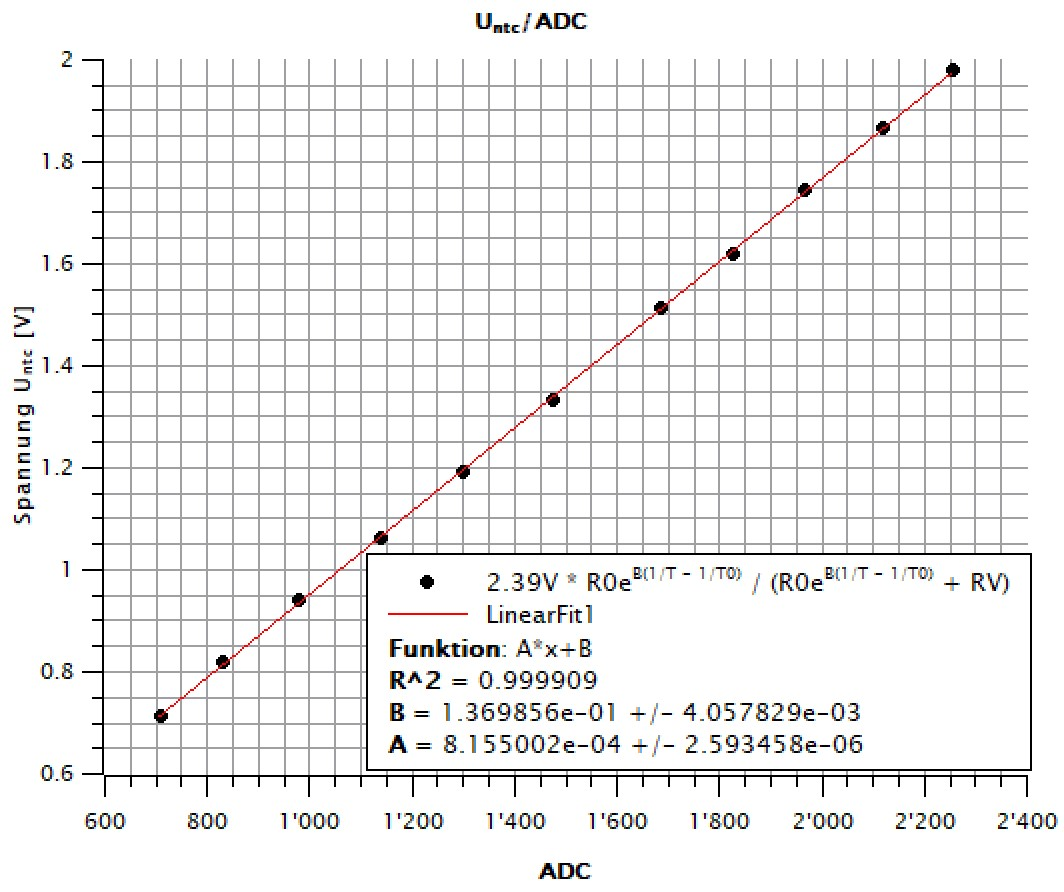
\includegraphics[width=0.9\textwidth]{graphics/Untc_ADC.jpg}
	\caption{$U_{ntc,berechnet}/ADC$}
	\label{pic: Untc_ADC}
\end{figure}

\begin{figure}[H]
	\centering
	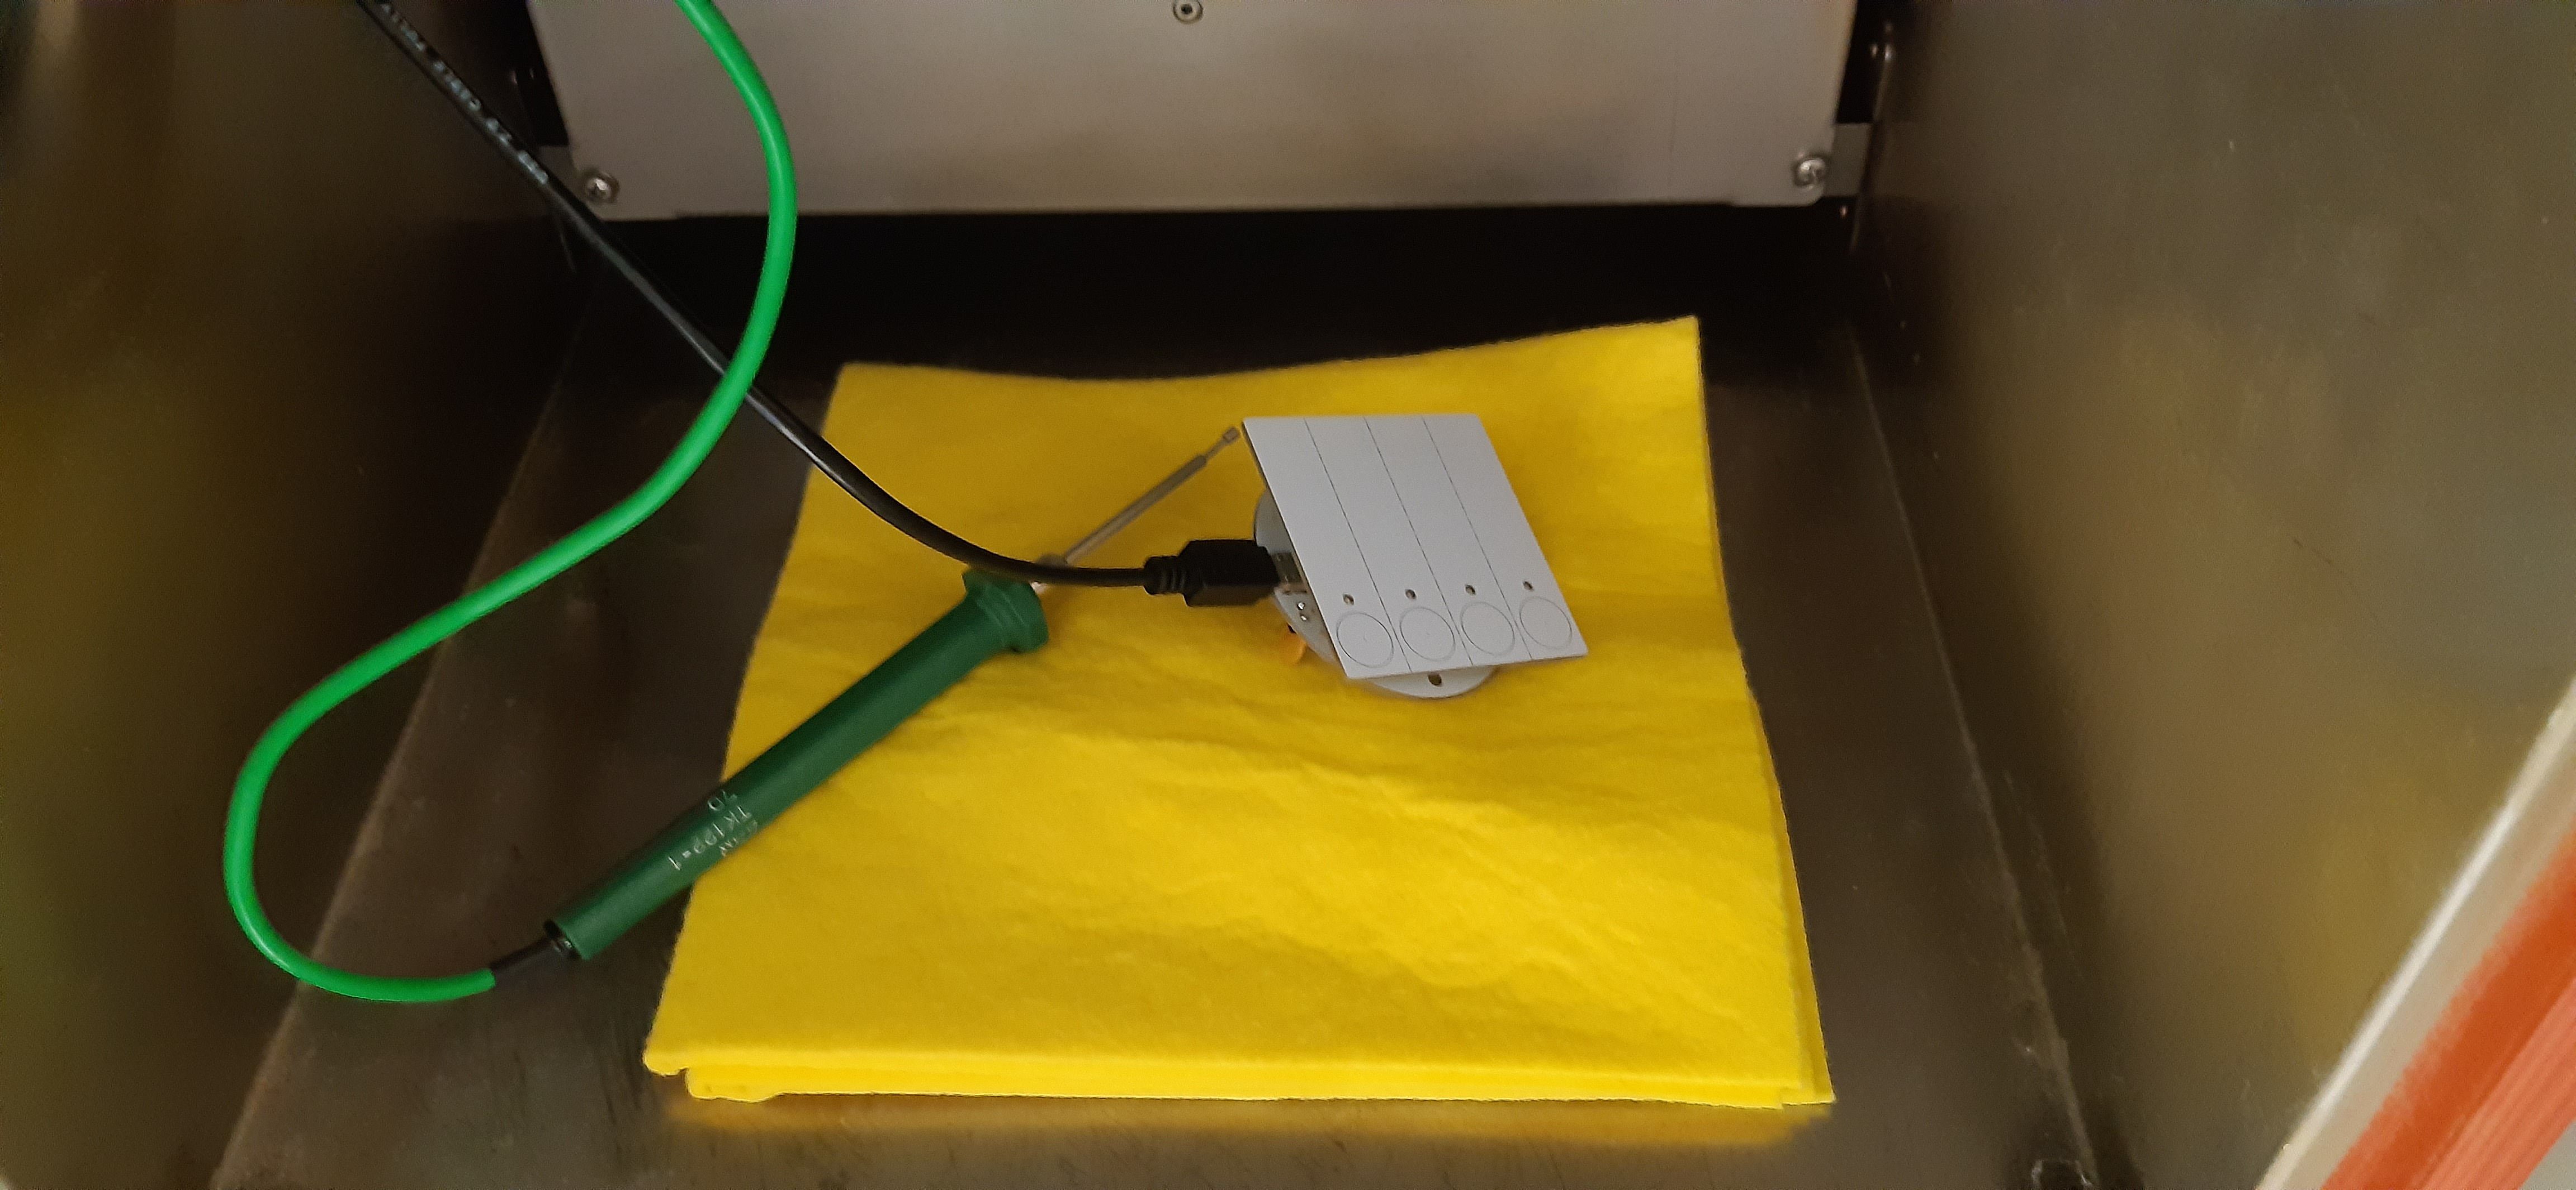
\includegraphics[width=0.90\textwidth]{graphics/Klimaschrank.jpg}
	\caption{Temperaturmessung im Klimaschrank}
	\label{pic: Klimaschrank}
\end{figure}

\newpage
\subsection{Programmcode Aktorbord}
Die Aufgabe des Aktorbord besteht darin, dass Befehle empfangen, verarbeitet und ausgeführt werden. Es befinden sich vier Relais auf dem Bord,welche 230 Volt schalten können, diese werden mit Digitalen IO Pins angesteuert. Eine weitere Aufgabe ist die Ausgabe von zwei DC-Spannnugen 0-10 Volt. Die jeweilige Spannung entsteht durch ein PWM Signal. Eine letzte Aufgabe ist, 0-10 Volt einlesen. Das Eingangssignal gelangt über ein Spannungsteiler an den AD-Wandler. Der Mikrocontroller wertet das Signal aus und generiert eine MQTT-Message welche in einem Periodischen Zyklus publishd wird.    


\subsubsection{	Übersicht} 
\begin{figure}[H]
	\centering
	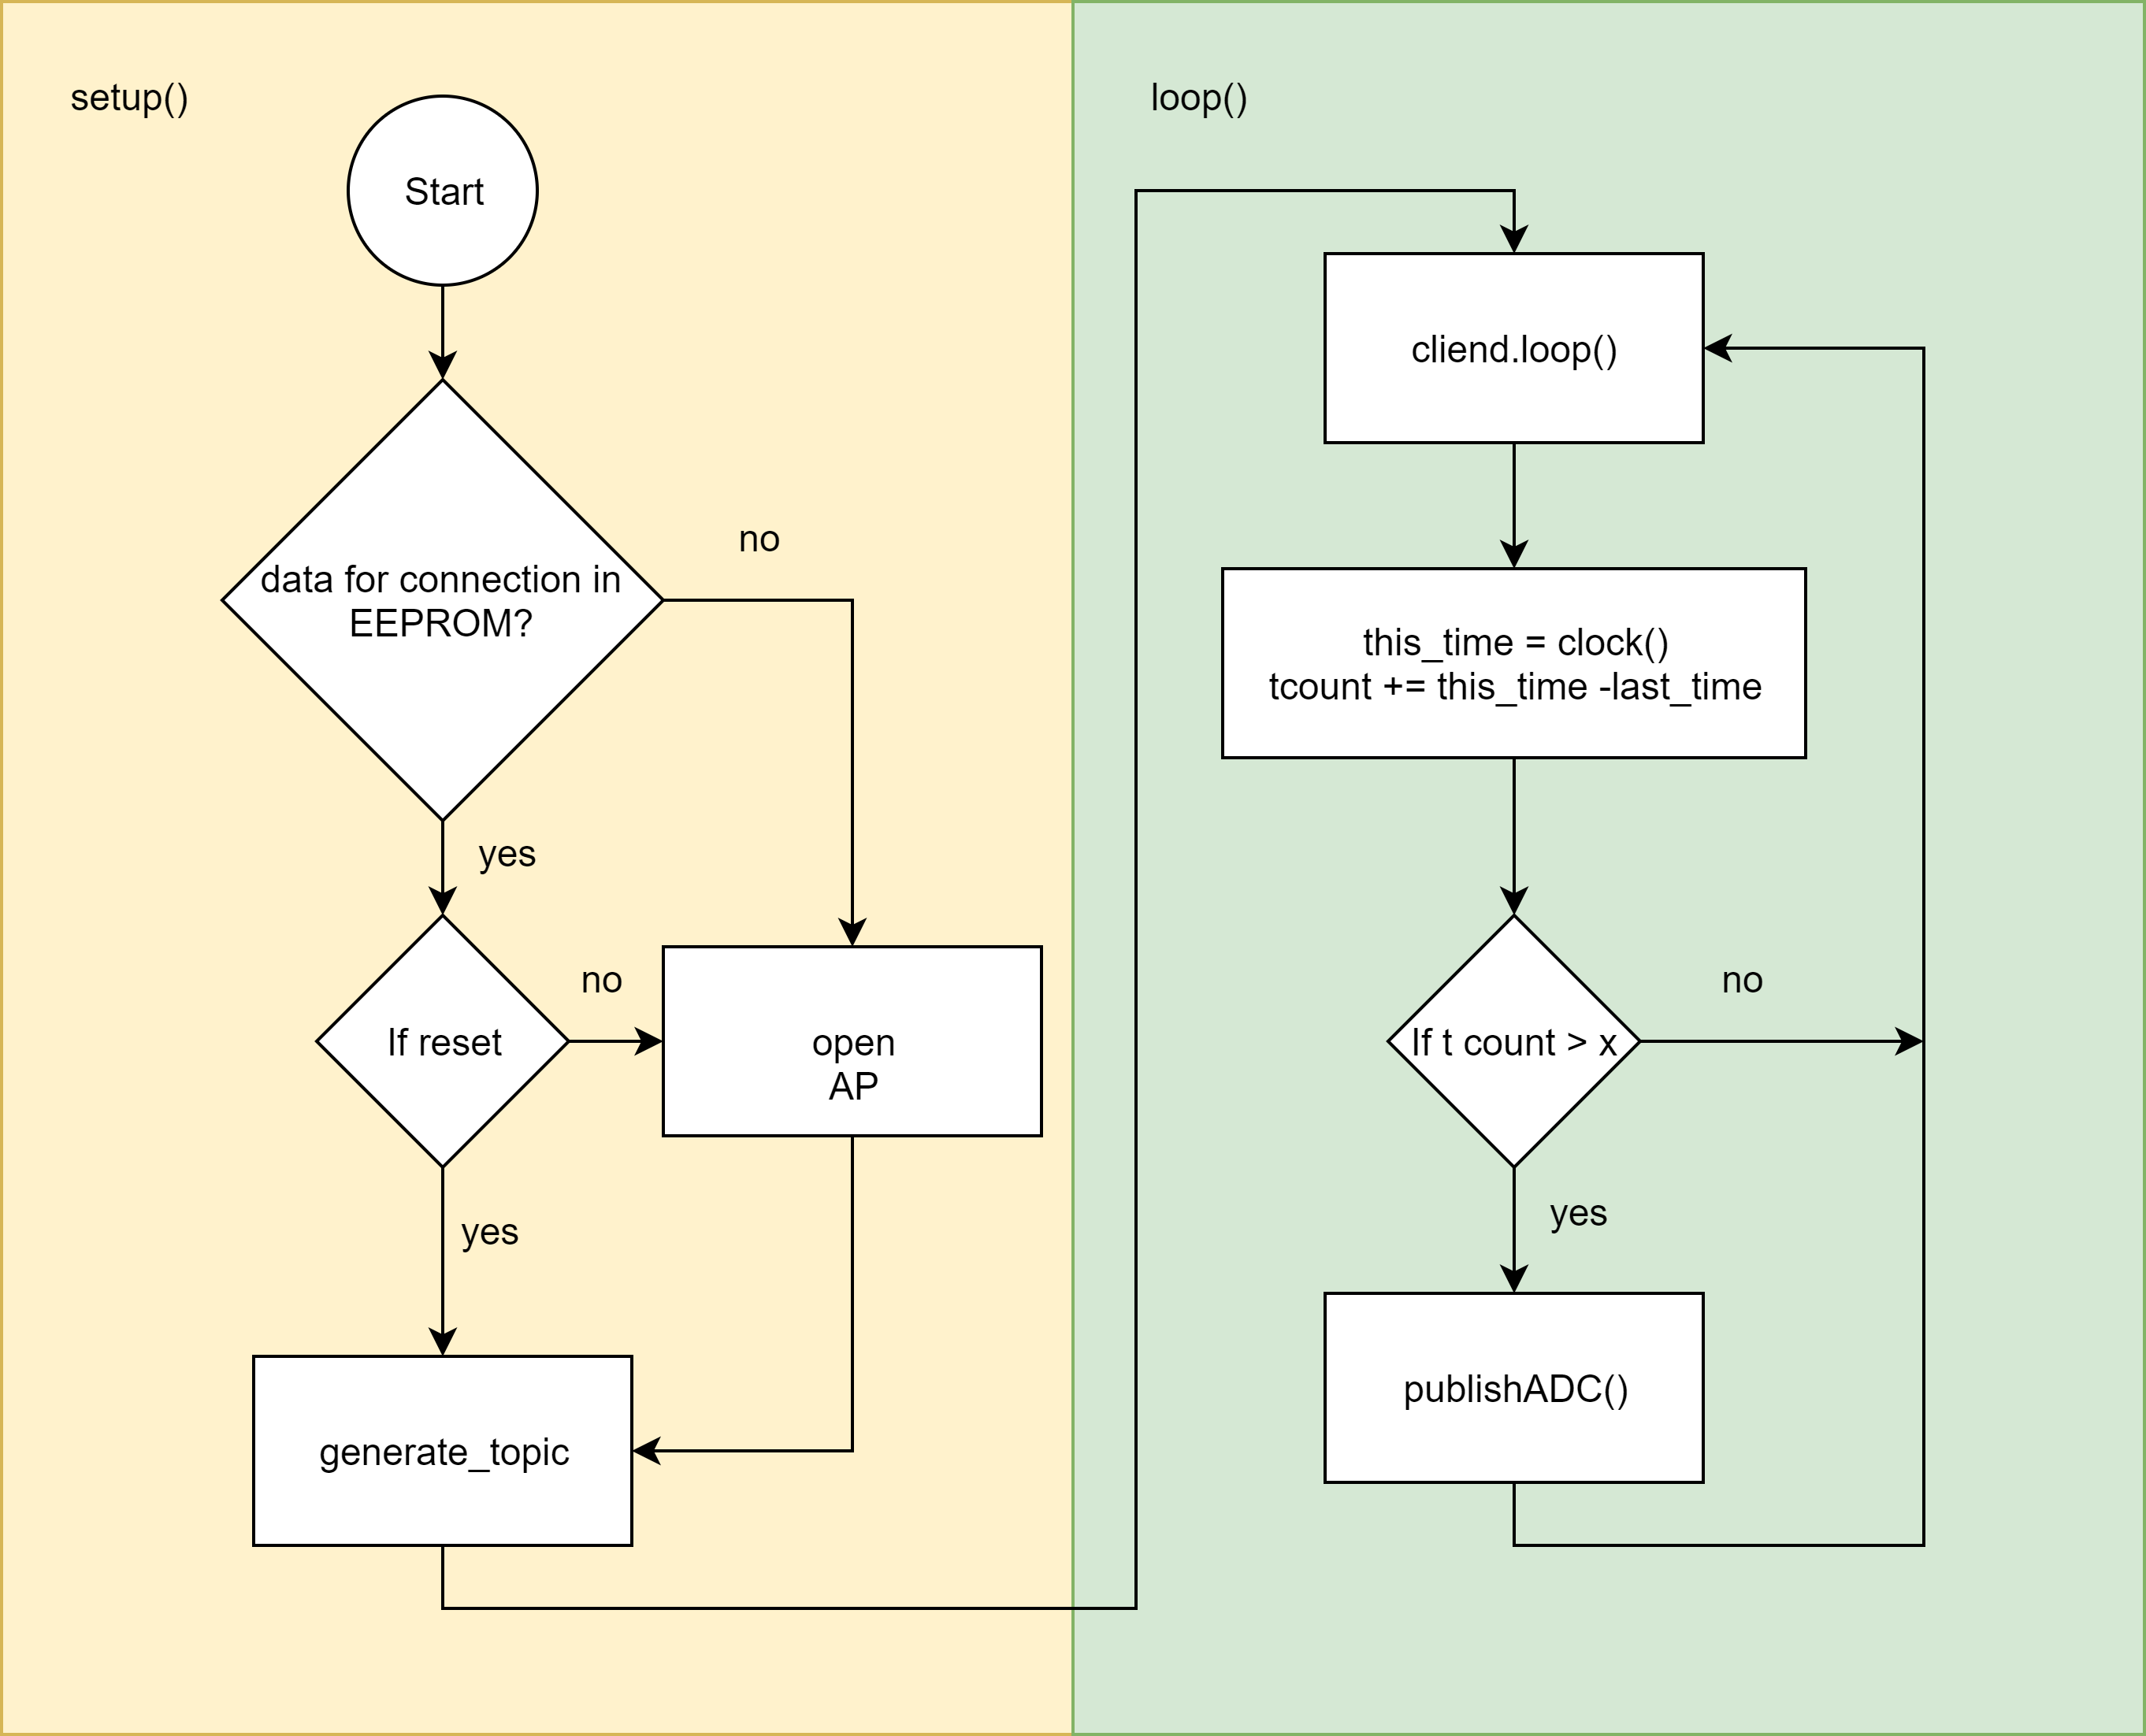
\includegraphics[width=\textwidth]{graphics/StatemaschineAktor.png}
	\caption{In dieser Abbildung ist das Statediagram vom Aktorbord abgebildet}
	\label{pic: statemaschine Aktor}
\end{figure} 
\newpage

\subsubsection{setup()}
In der Abbildung ist zu erkennen, dass genau der gleiche Ablauf wie beim Sensorprint \ref{subsubsec: sensor setup} statt findet. Wird aber der Programm Code selber betrachtet werden andere Bezeichnungen wie andere Definitionen von pinMode() usw. im Bezug zum Sensorbord Festgestellt werden. 
\subsubsection{loop()}
Im loop() wird als erstes die Funktion clien.loop() aufgerufen. Diese Funktion ist im wesentlichen zuständig, dass MQTT Befehle empfangen und verarbeitet werden, Sie wird anschliessend ausführlich erläutert. In einem weiteren Schritt wird wie im loop() vom Sensorbord beschrieben \ref{subsubsec: sensorloop}, Periodischer Zyklus erstellt welche nur alle 10 Sekunden ausgeführt wird. In diesem Zyklus befindet sich die Funktion publishADC, welche die gemessenen Werte von den 0-10 Volt Eingenen als MQTT-Message published.
\begin{figure}[H]
	\centering
	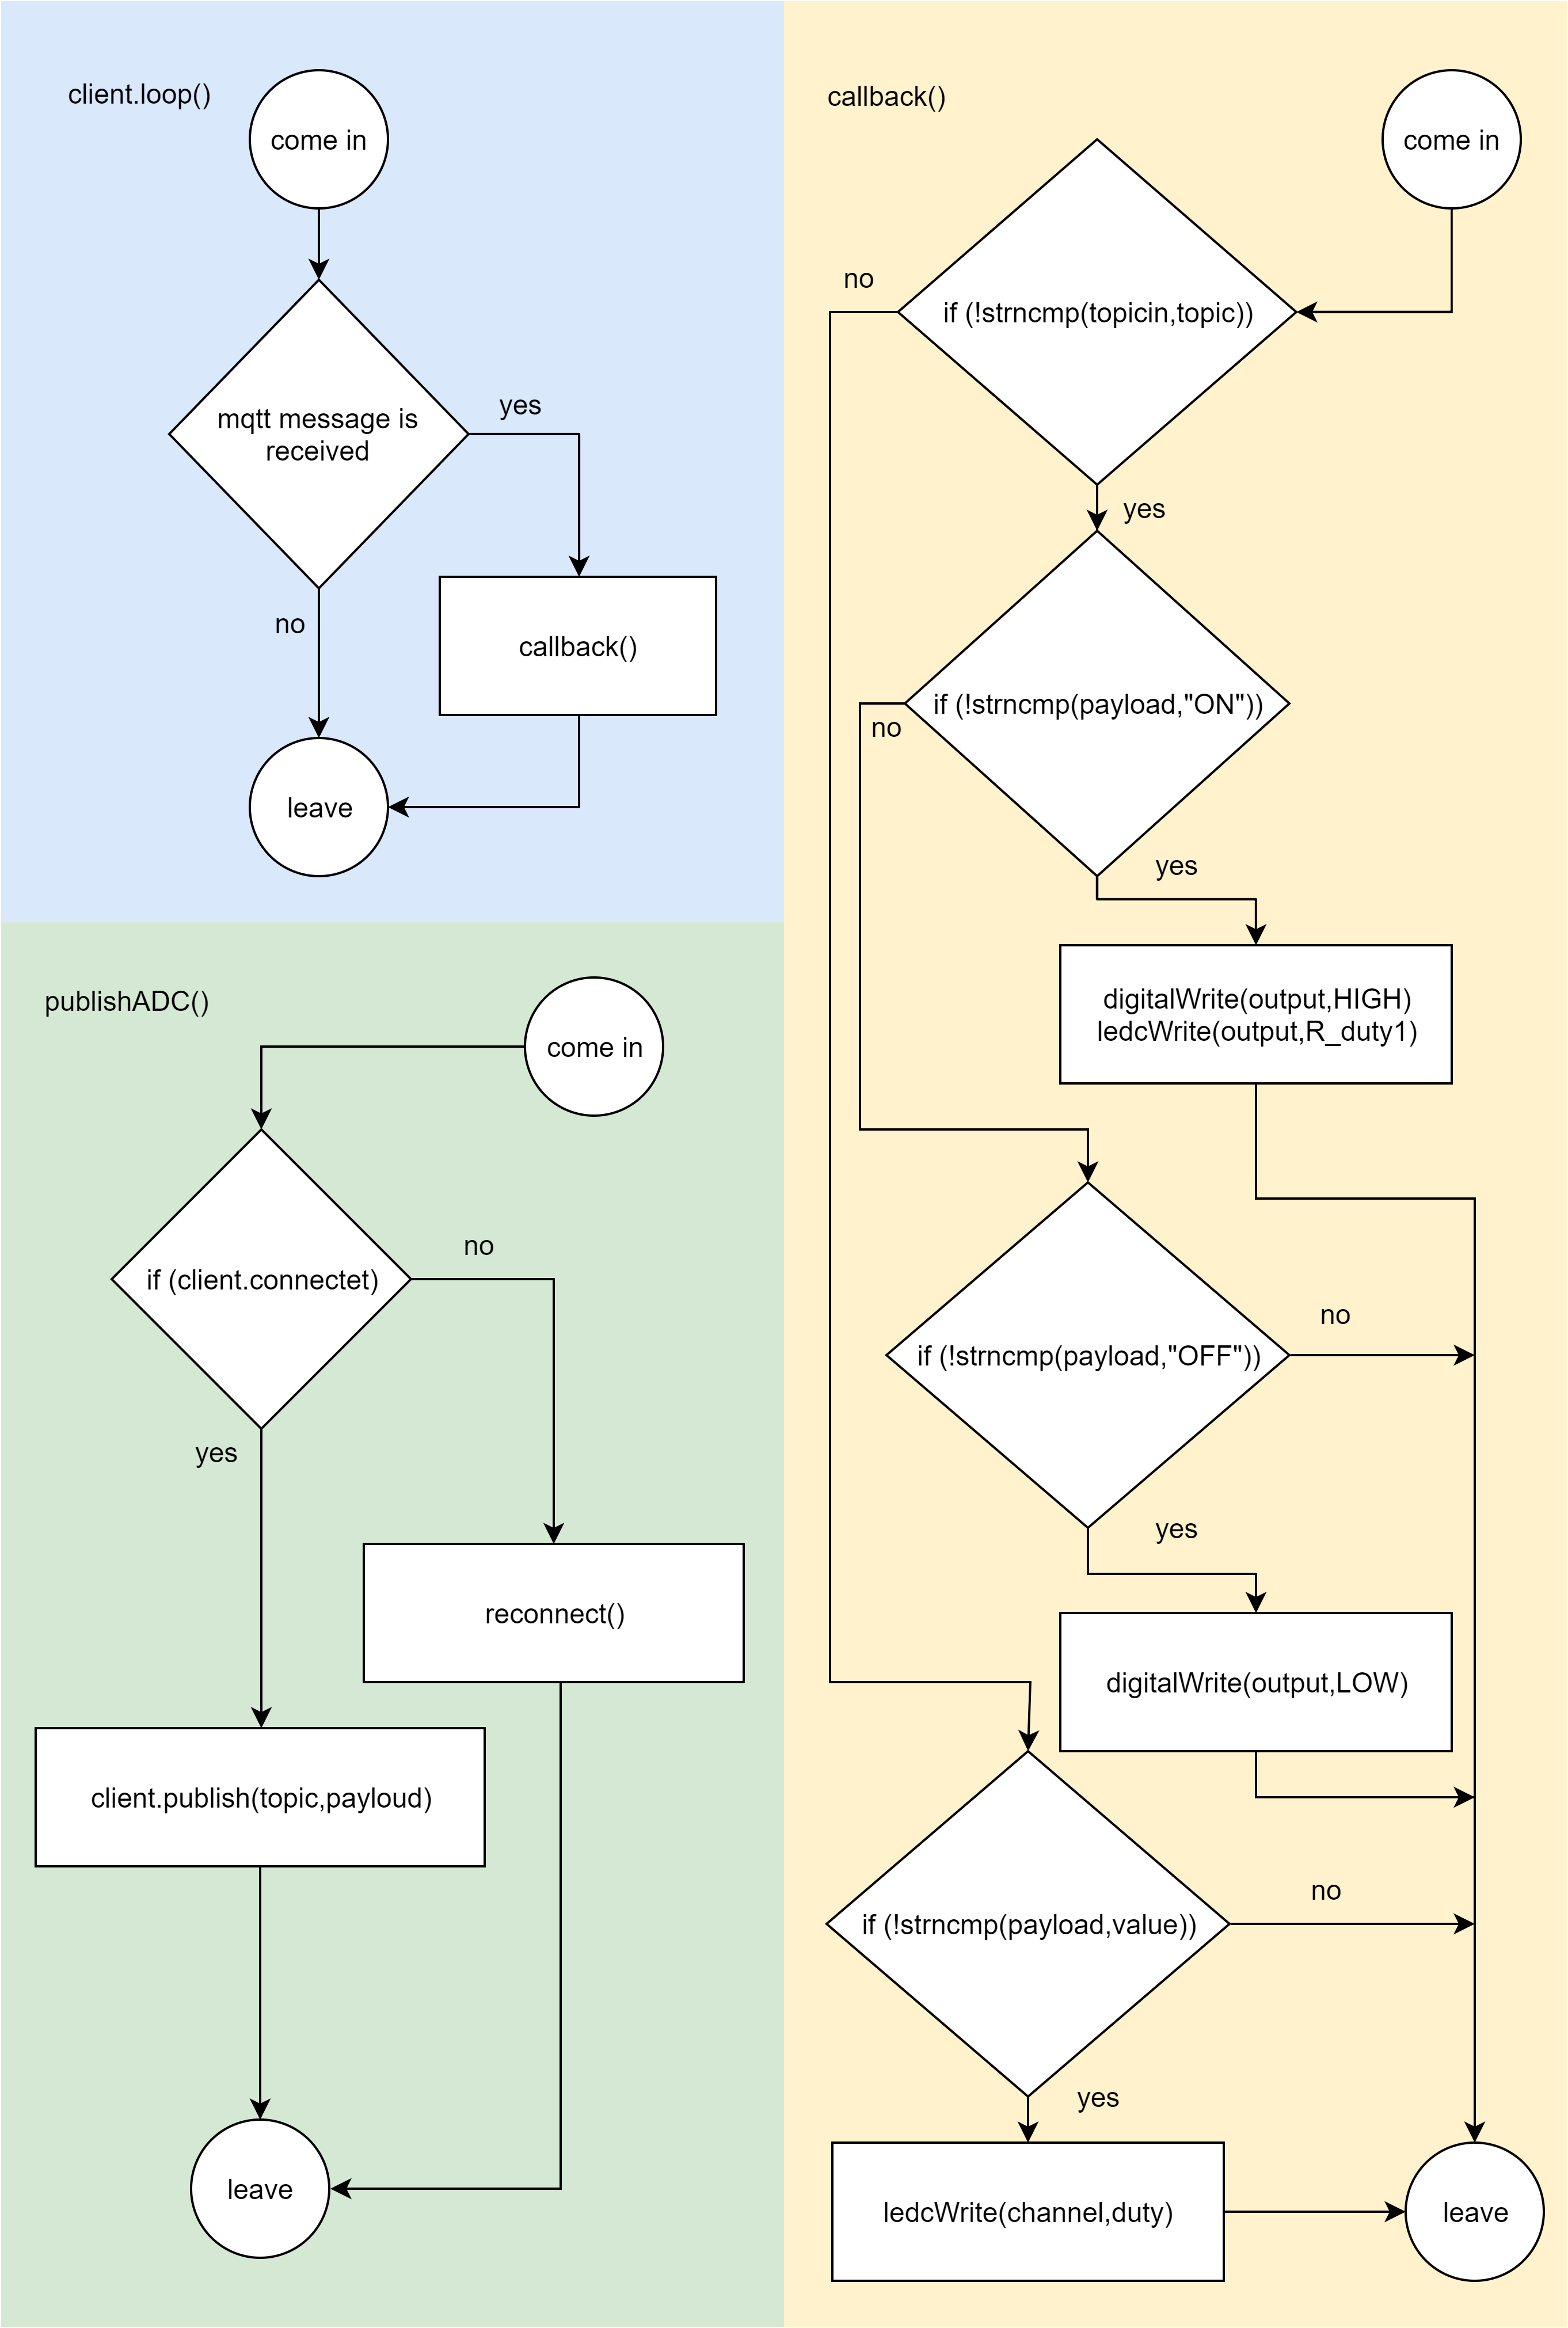
\includegraphics[width=\textwidth]{graphics/FunktionenAktor.png}
	\caption{In dieser Abbildung sind die Funktionen vom Sensorboard abgebildet}
	\label{pic: funktionen Aktor}
\end{figure}   
\subsubsection{client.loop()}
 Das Objekt \textit{client} wurde aus dem PubSubClient gebaut, wo der loop() implementiert wurde. Als erstes wird die Verbindung zum MQTT-Broker überprüft, dann bei bedarf die MQTT-Message empfangen und vorbereitet, dass sie in der Funktion callback()  genutzt werden kann. callback() wird aufgerufen.
 \subsubsection{callback()}
 In dieser Funktion wird als erstes der Inhalt von der Empfangenen Topic überprüft, fällt der Vergleich positiv aus wird der Inhalt der Payload überprüft. Die vier Verschiedenen Relais und die zwei Analogausgänge unterscheiden sich an Hand der Topic. Bei den Relais ist die Payload ON oder OFF und das Relais wie auch das Led des entsprechenden Relais wird in den geforderten zustand gesetzt. Trift die Topic auf ein Analog Ausgang wird nach Umwandlung der Payloud von einem String in ein Float, das PWM-Signal für den entsprechenden Ausgang gesetzt. Den Duty cycle für das PWM Signal wird berechnet indem die gewünschte Spannung voltage folgender Massen verrechnet wird : $(voltage/3.2 \cdot 4095)/3.25$. 3.2 sind es, weil die Verstärkung 3.2 beträgt und 3.25, weil das die Amplitude des PWM Signales ist. Leider kann die Amplitude abweichen und ist nicht sehr genau. Mehr zur Genauigkeit in der Validierung.
 
 \subsubsection{publishADC()}
Mit dieser Funktion werden die 0-10 Volt Eingänge ausgewertet und Resultate als MQTT-Message versendet. Der jeweiligen Messreihe am ADC wird der Mittelwert berechnet, welcher dann von einem float in ein char-Array umgewandelt wird. Als nächstes wird der char-Array und die entsprechende Topic vom PupsubClient veröffentlicht.

\subsection{Task2code()}
Diese Funktion wird im Gegensatz zum Rest des Programms im zweiten Kernel des ESP32 verwendet. Falls ein Relais in der Callback() Funktion gesetzt wird, wird in dieser Funktion die Zeit gemessen und nach 25\,ms wird der Sparmodus für das jeweilige Relais gesetzt. Das setzten des Sparmodus passiert für alle Relais einzeln, es spielt keine Rolle wann ein Relais gesetzt wird, es dauert immer 25\,ms $\pm 3 \,ms$. Der zweite Kernel ist somit nur damit beschäftigt, zu prüfen ob ein Relais aktiviert wurde und es dann nach einer vordefinierten Zeit in den Sparmodus zu bringen.
\newpage

\subsection{Programmcode Openhab}        
Der Aufbau des Systems besteht aus verschiedenen Komponenten welche in nachfolgender Tabelle aufgelistet sind
\begin{table}[H]
	\begin{tabular}{|l|l|}
		\hline 
		Bezeichnung	& Beschreibung \\ 
		\hline 
		Bindings	& Schnittstellen verknüpft verschiedene Dienste miteinander  \\ 
		\hline 
		Things	& Definition von Gerät, Verbraucher, Teilnehmer des Systems  \\ 
		\hline 
		Channel	& Verbindung zwischen Thing und Item  \\ 
		\hline 
		Item	& Repräsentiert Informationen des Gerätes, Schalter, Label usw. \\ 
		\hline 
		Rules	& Festgelegte Regeln für automatische Abläufe\\ 
		\hline 
		Sitmaps	& Benutzeroberfläche, präsentiert Informationen  \\ 
		\hline 
	\end{tabular} 
	\caption{Komponenten Openhab Software \cite{noauthor_introduction_nodate-1}}
	\label{tab: Komponenten Openhab Software}
\end{table}
\begin{figure}[H]
	\centering
	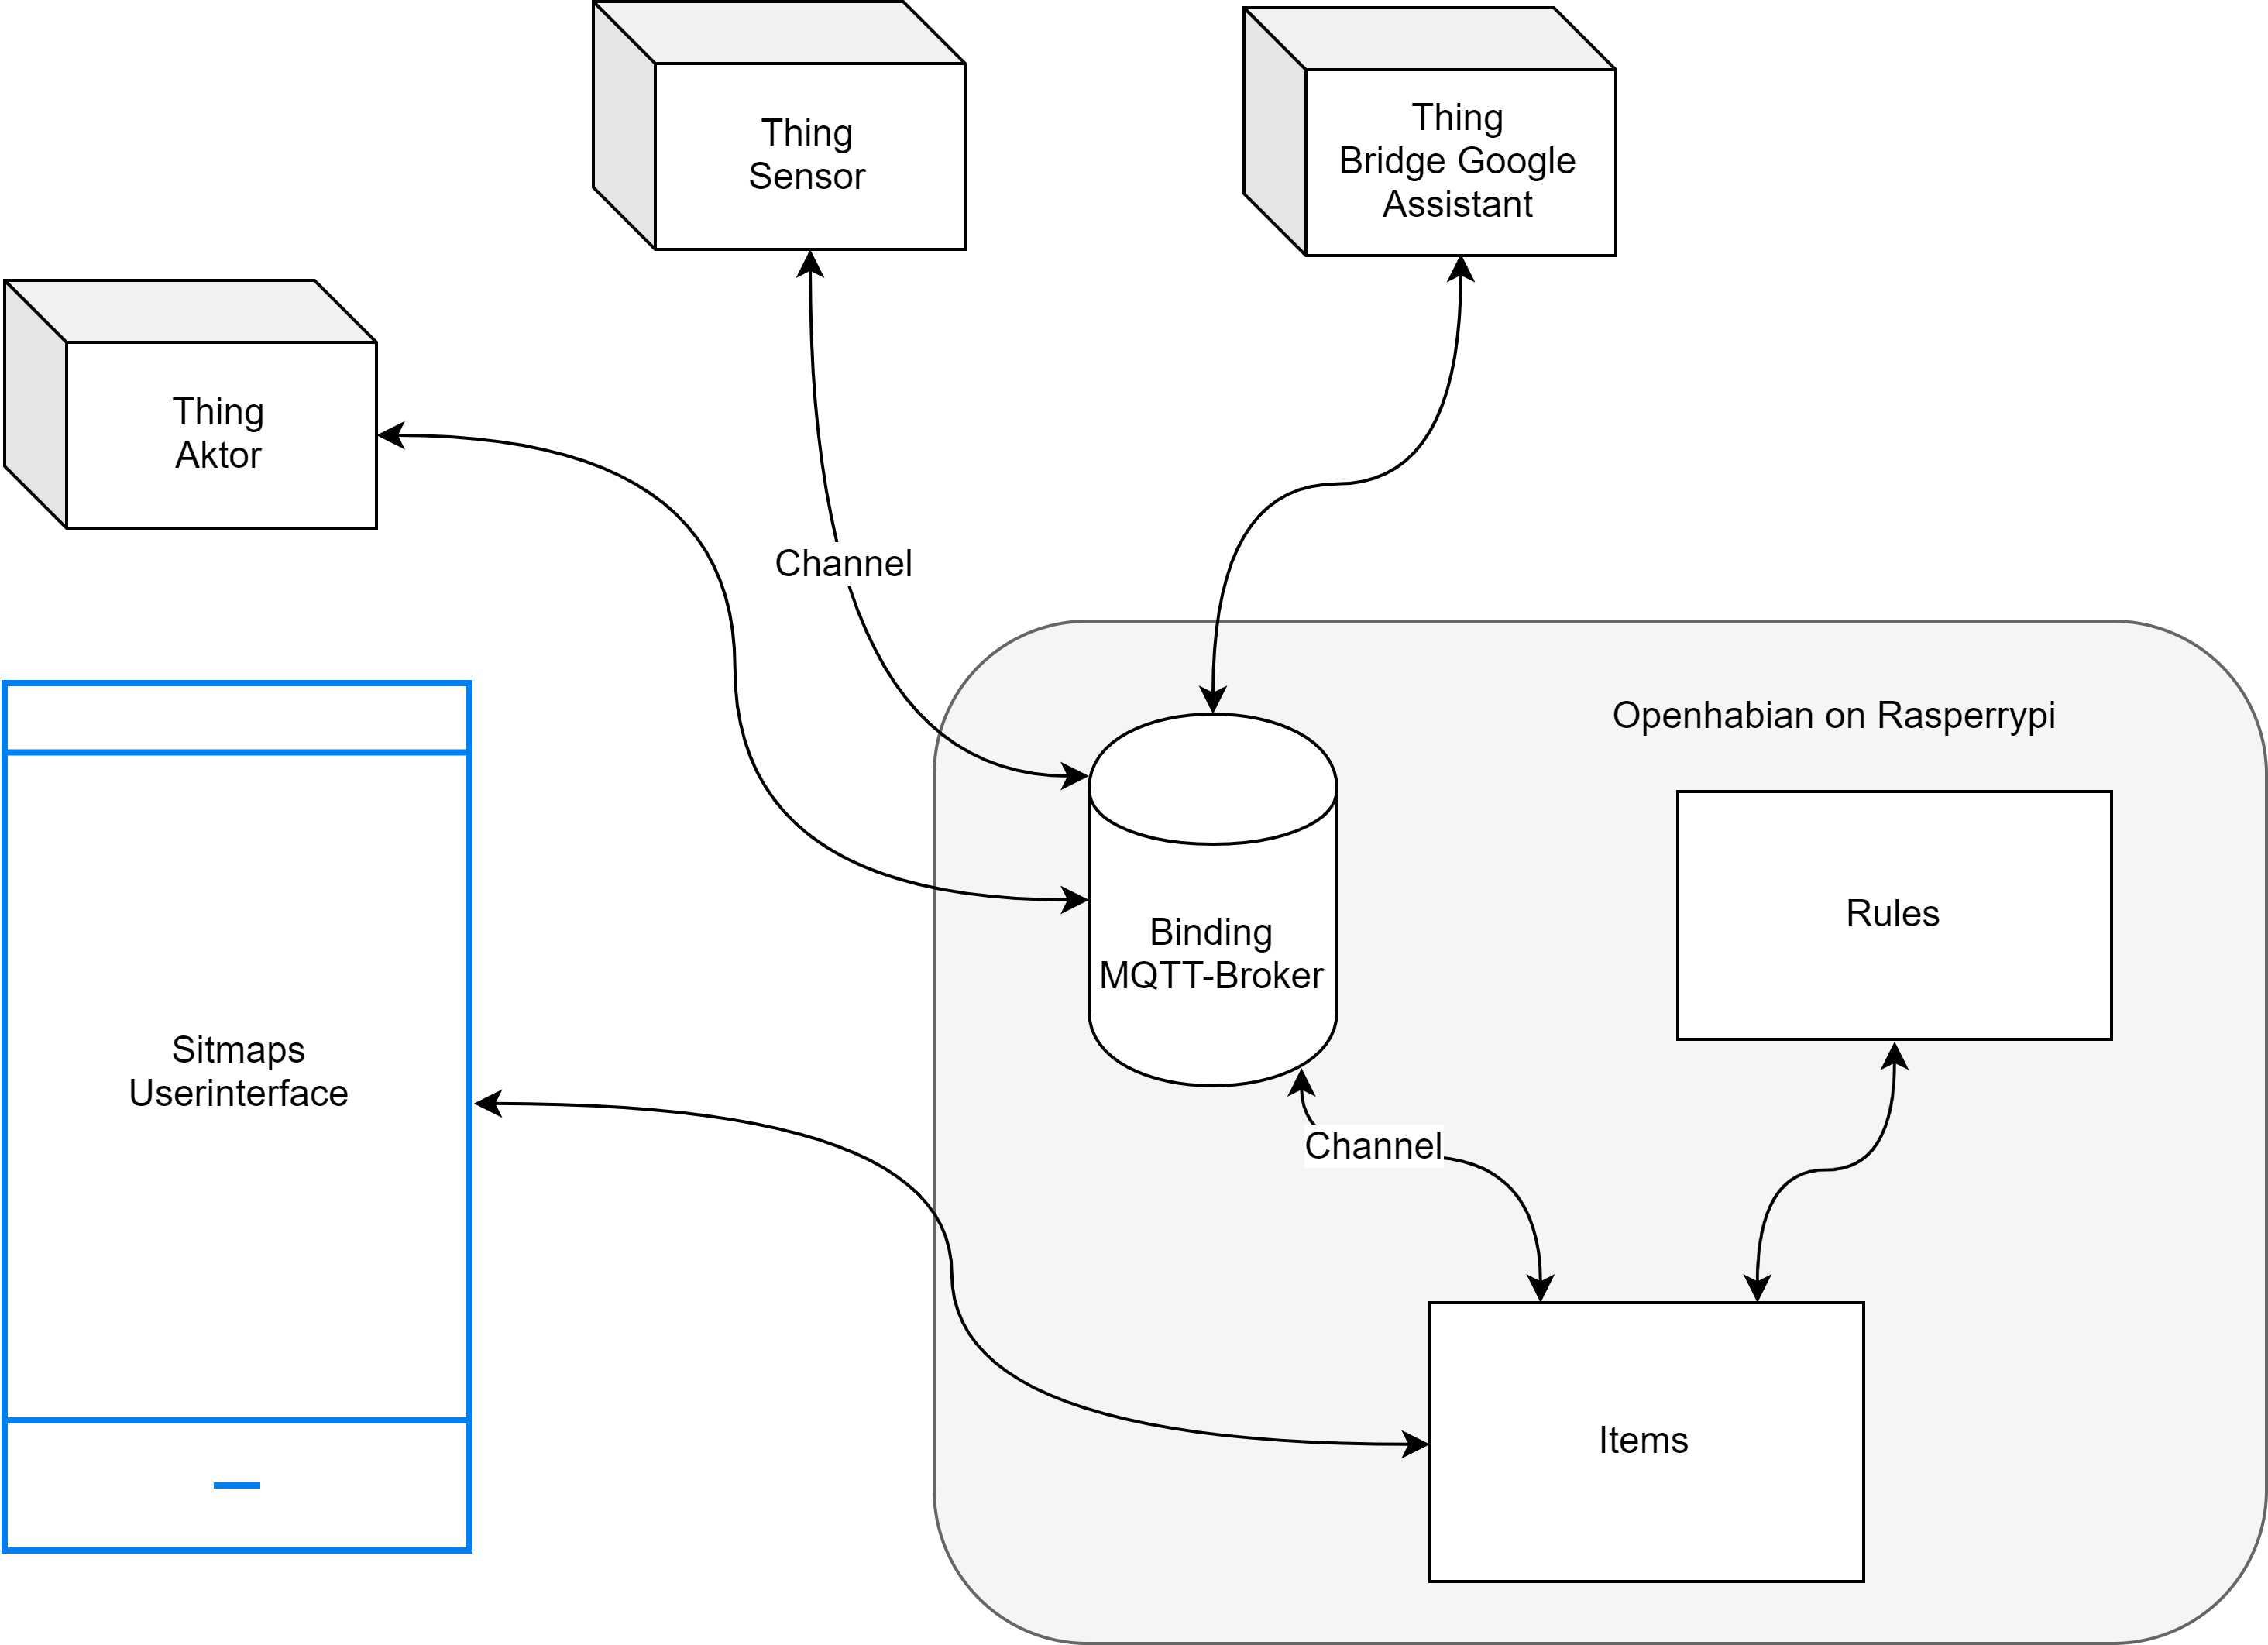
\includegraphics[width=\textwidth]{graphics/Openhabian.png}
	\caption{Komponenten und Verbindungen von Openhab}
	\label{pic: Komponenten Openhab}
\end{figure}   

\subsubsection{Bindings}
Als Schnittstelle von den Items zu den Things wird ein MQTT-Broker benötigt. Um die Systemzuverlässigkeit zu steigern wurde ein eigener Broker Installiert, so kann die Kommunikation auch ohne Netzwerkanschluss ans Öffentliche Netz funktionieren. Ein weiterer Vorteil ist die Sicherheit, es kann auf Passwörter verzichtet werden, da kein Zugriff von ausserhalb des Home-Netzwerk möglich ist.

\subsubsection{Things}
 Als Geräte wurden drei Komponenten hinzugefügt, welche in der Abbildung \ref{pic: Komponenten Openhab} zu erkennen sind. Zum Aktor Thing gelangen im ganzen 8 Channels, um die Relais einzeln anzusprechen wurde pro Relais eine MQTT-Topic erstellt welche je einen Channel verfügt und so mit je einem Item verbunden. Zwei Channel sind für die 0-10 Volt Eingänge und zwei weiter Channel für die 0-10 Volt Ausgänge. Das Sensor Thing verfügt 5 Channel jeder Taster einzeln und ein Channel für die Temperaturmessung.

\subsubsection{Channel}
Die Channes sind die Verbindungen von den Geräten zu den Items also den Software-Zustände, in diesem Projekt werden alle möglichen Fähigkeiten der Geräte genutzt und mit einem Channel gebunden.

\subsubsection{Item}
Das Item zeigt den Status des Verbrauchers oder den gemessenen Wert eines Sensors an. Items werden verwendet wenn Regeln definiert werden,ebenso sind sie mit den Channels verlinkt und können einzeln oder als Gruppen auf dem Sitmap genutzt werden. Als anwendung eines Icons können verschiedene Typen gewählt werden. In diesm Projekt wird in erste Linie der normale Switch verweden welcher in den Zustand ON oder OFF geschalten wird. Für die 0-10 Volt ausgänge werden Dimmer verwendet die als Slider in der Sitmap angezeigt wird und Sie generieren je nach Position einen Wert zwischen 0-1. Um die Messwerte an den 0-10 Volt Eingängen zu verwenden werden die Items als Number genutzt.

\subsubsection{Rules} 
Automatische Prozesse werden mit i Rules definiert. Um das System Benutzerfreundlicher zu Gestalten werden in den Rules die Befehle der Taster verarbeitet und die Entsprechenden Befehle an die Relais generiert. So kann gewährleistet werden, dass der Kunde selber keine Änderungen an den Aktoren und Sensoren selber vornehmen muss. Die Rule Syntax basiert auf Xbase \cite{noauthor_xtext_nodate}. Um die Aufgeben der Befehls Weiterleitung zu übernehmen bestehen die Ruls im wesentlichen aus when und then. In diesem Fall sind sie im Teil when, auf den Empfang des jeweiligen Update getriggert. Somit wird mit einem Update des Status der Teil then ausgelöst, wo sich eine if Bedingung befinden. In diese Bedingung wird der Stus überprüft      

\subsubsection{Sitemaps} 
Als Sitemaps wird das Userinterface bezeichnet. Auf einer Sitemap  gibt es die Möglichkeit verschiedene Elemente in Form von Frame, Text oder Schalter darzustellen, diese Elemente präsentieren Status und Informationen vom System. Das Frame ist Beispielsweise die Aufteilung von einem Haus in seine einzelnen Stockwerke. In den einzelnen Stockwerken werden dann Schalter für jeweilige Geräte als Item hinzugefügt. Mehrere Schalter können als Gruppe zusammen gefasst werden, so kann in zentral Schalter ein/aus realisiert werden. Das erstellte Sitmap ist im Webbrowser mittels IP-Adresse des Servers oder mit dem Openhab Mobile-App erreichbar.

